% latex article template

% cheat sheet(eng): http://www.pvv.ntnu.no/~walle/latex/dokumentasjon/latexsheet.pdf
% cheat sheet2(eng): http://www.pvv.ntnu.no/~walle/latex/dokumentasjon/LaTeX-cheat-sheet.pdf
% reference manual(eng): http://ctan.uib.no/info/latex2e-help-texinfo/latex2e.html

% The document class defines the type of document. Presentation, article, letter, etc. 
%\documentclass[12pt, a4paper]{report}
\documentclass[pdftex,10pt,b5paper,twoside]{book}

% packages to be used. needed to use images and such things. 
\usepackage[hidelinks, pdfborder=0 0 0]{hyperref} % pdf properties ++
\usepackage[utf8]{inputenc}
\usepackage[english]{babel}
\usepackage{graphicx} % pictures thingy
\usepackage{glossaries}
\usepackage[options]{natbib} % bibliography thing.
\usepackage{hyphenat}
\PassOptionsToPackage{hyphens}{url}
%\usepackage{listing}
\usepackage{listings} % syntax thing
\usepackage{color}
\usepackage{setspace}

% import syntax highlighting
% python syntax. 
% http://widerin.org/blog/syntax-highlighting-for-python-scripts-in-latex-documents

\definecolor{Code}{rgb}{0,0,0}
\definecolor{Decorators}{rgb}{0.5,0.5,0.5}
\definecolor{Numbers}{rgb}{0.5,0,0}
\definecolor{MatchingBrackets}{rgb}{0.25,0.5,0.5}
\definecolor{Keywords}{rgb}{0,0,1}
\definecolor{self}{rgb}{0,0,0}
\definecolor{Strings}{rgb}{0,0.63,0}
\definecolor{Comments}{rgb}{0,0.63,1}
\definecolor{Backquotes}{rgb}{0,0,0}
\definecolor{Classname}{rgb}{0,0,0}
\definecolor{FunctionName}{rgb}{0,0,0}
\definecolor{Operators}{rgb}{0,0,0}
\definecolor{Background}{rgb}{0.98,0.98,0.98}

\lstnewenvironment{python}[1][]{
\lstset{
numbers=left,
numberstyle=\footnotesize,
numbersep=1em,
xleftmargin=1em,
framextopmargin=2em,
framexbottommargin=2em,
showspaces=false,
showtabs=false,
showstringspaces=false,
frame=l,
tabsize=4,
% Basic
basicstyle=\ttfamily\small\setstretch{1},
backgroundcolor=\color{Background},
language=Python,
% Comments
commentstyle=\color{Comments}\slshape,
% Strings
stringstyle=\color{Strings},
morecomment=[s][\color{Strings}]{"""}{"""},
morecomment=[s][\color{Strings}]{'''}{'''},
% keywords
morekeywords={import,from,class,def,for,while,if,is,in,elif,else,not,and,or,print,break,continue,return,True,False,None,access,as,,del,except,exec,finally,global,import,lambda,pass,print,raise,try,assert},
keywordstyle={\color{Keywords}\bfseries},
% additional keywords
morekeywords={[2]@invariant},
keywordstyle={[2]\color{Decorators}\slshape},
emph={self},
emphstyle={\color{self}\slshape},
%
}}{}


% hides the section numbering. 
%\setcounter{secnumdepth}{-1}

% Graphics/image locations and extensions. 
\DeclareGraphicsExtensions{.pdf, .png, .jpg, .jpeg}
\graphicspath{{./images/}}

% Commands
\renewcommand{\arraystretch}{1.2}

% Author, title and type
% Used in the title page. 
\newcommand{\thesisAuthor}{Magnus L. Kirø}

%TODO revise thesis title. 
\newcommand{\thesisTitle}{
Tweet Sentiment, Sentiment Trend, and a Comparison with Financial Trend Indicators.
%Sentiment analysis of Tweets in correlation with financial investments
}
\newcommand{\thesisType}{Masters Thesis}
\newcommand{\thesisKeywords}{Twitter, Sentiment, Sentiment Analysis, SVM, Naive
Bayes, NLP, Finance, Stock market prediction, Moving Average, Trading, Average
Directional Index, Trend, Trend Analysis, Trend Prediction}

% setting the embedded pdf metadata. Visible under pdf properties in your
% viewer. 
\hypersetup{
    pdfauthor={\thesisAuthor},
    pdftitle={\thesisTitle},
    pdfsubject={\thesisType},
	pdfkeywords={\thesisKeywords},
    pdfnewwindow=true,
    colorlinks=true,
    linkcolor=black,
    filecolor=red,
    urlcolor=blue,
    citecolor=magenta
}

% beginning of the document content, end of the configuration and setup. 
\begin{document}

% pretexts: title page, abstract, metadata, acknowledgements, toc, lot, lof  
\clearpage
\pagenumbering{roman} 				
\setcounter{page}{1}

\pagestyle{fancy}
\fancyhf{}
\renewcommand{\chaptermark}[1]{\markboth{\chaptername\ \thechapter.\ #1}{}}
\renewcommand{\sectionmark}[1]{\markright{\thesection\ #1}}
\renewcommand{\headrulewidth}{0.1ex}
\renewcommand{\footrulewidth}{0.1ex}
\fancypagestyle{}{\fancyhf{}\renewcommand{\headrulewidth}{0ex}}

% front page, contains: title, author, institution, and logo
%\begin{titlepage}
    \noindent {\large \textbf{\thesisAuthor} \small \today}
    \vspace{2cm}

\nohyphens{ 
    \noindent {\Huge \thesisTitle}
    \vspace{2cm}
}

    %TODO removed on completion
    \noindent {
        \Huge \textbf{Work in progress},
        \\ \Large to be completed by 1. jun 2014.
        \\ \url{https://github.com/magnuskiro/master
    }
    \vspace{2cm}
    % end todo remove. 

    \noindent \thesisType, \date{\today}
    \vspace{2cm}

    \noindent
    Artificial Intelligence Group\\
    Department of Computer and Information Science\\
    Faculty of Information Technology, Mathematics and Electrical Engineering\\

    \vfill
    \begin{center}
        
\includegraphics[]{NTNUlogo}
    \end{center}
\end{titlepage}



\noindent

% abstract
\section*{\Huge Abstract \small{English}}
\addcontentsline{toc}{chapter}{Abstract}
$\\[0.1cm]$
\begin{abstract}\label{abstract}

\paragraph{Background:}
As Twitter has become a global microblogging site, it's influence in the stock
market has become noticeable. This makes tweets an interesting medium for
gathering sentiment. A sentiment that might influence trends in the stock
market. 

\paragraph{Motivation:} 
If Twitter can be used to predict future prices in the stock market
the casual investor would gain an advantage over the day-trader and the modern trading algorithms. 

Another interesting aspect is the role of Twitter in sentiment
analysis. And how Twitters role as a data source influences trends in the stock
market.   

\paragraph{Data and Experiments:} 
Twitter is used as the data source. It provides easy access, lots of data, and
many possibilities to use available metadata. 
To find the sentiment of a tweet we use two methods, counting positive and
negative words(bag of words), and classifiers (SVM and Naive Bayes). 
We use moving average(MA) and average directional index(ADX) as trend
indicators. We calculate MA and ADX with data from Oslo stock exchange, and we
created our own indicators, based on MA and ADX, using data from Twitter. Then we
compare the graphs.  

\paragraph{Findings:}
We explore the usage of lists of words, dictionaries, in sentiment analysis.
And we look at data retrieval from Twitter and the trend we can create from it.
To a varying degree we get positive results with the dictionaries, while the
trend aggregation lacks the finesse and results we hoped for.

\paragraph{Conclusion:} 
Sentiment classification of tweets worked with both bag of words, and trained
classifiers. We also managed to aggregate a trend based on sentiment, but we
found no correlation between the financial trend indicators and the sentiment indicators. 

\end{abstract}


%\clearpage

% abstract norwegian version
%\section*{\Huge Abstrakt \small{Norwegian}}
\addcontentsline{toc}{chapter}{Abstrakt}
$\\[0.1cm]$
\begin{abstract}\label{abstract-nor}


\paragraph{Bakgrunn:}
Siden Twitter har blitt et globlat nettsted for mikroblogging har innflytelsen
til Twitter i aksjemarkedet bitt betydelig. 
Dette gjør tweets til et interessant medium for å samle sentiment. Et sentiment
som potensielt kan påvirke utviklingen i aksjemarkemarkedet.

\paragraph{Motivasjon:}
Hvis Twitter kan brukes til å forutsi trender i aksjemarkedet vil den alminnelige
investor få en fordel over en intra-dag trader eller de moderne
trading-algoritmene. Et annet interessant aspekt er rollen til Twitter i sentiment
analyse, og hvordan Twitter sin rolle som datakilde påvirker utviklingen i
aksjemarkedet.

\paragraph{Data og Eksperimenter:}
Twitter brukes som datakilde og gir enkel tilgang, mye data, og mange
muligheter til å bruke tilgjengelige metadata. For å finne sentimentet av
en tweet bruke vi 'bag of words', SVM, og Naive Bayes. For finans delen og
sammenligning av trendene bruker vi data fra Oslo Børs. Vi bruker 'moving
average'(MA) og 'average directional index'(ADX) som trend
indikatorer. Trend sammenligningen er basert på MA og ADX. Vi beregner MA og ADX
med finansdata, og sentiment data basert på tweets. Deretter sammenligner vi
grafene.

\paragraph{Funn:}
Vi utforsker bruken av lister med ord, ordbøker, i sentiment analyse. Og vi ser
på innhenting av data fra Twitter og trenden vi kan lage med dataene. I
varierende grad får vi positive resultater med ordbøkene, mens trend aggregering
mangler finesse, og kvaliteten den burde ha hatt.

\paragraph{Konklusjon}
Sentiment klassifisering av tweets fungerte med begge metodene. Vi klarte å
aggregere en trend basert på sentiment. Men sammenligningen med finans trendene
fungerte ikke som vi håpet. Ingen likheter ble funnet mellom sentiment trenden
og finans trenden.

\end{abstract}

%\clearpage

% metadata
\begin{abstract}\label{metadata}

Metadata ?

github repository for code an thesis. 

word count for fun. 


\end{abstract}

\clearpage

% Acknowledgements 
\begin{abstract}\label{acknowledgements}
Acknowledgements goes here. 
% todo write thanks to all the ocntributors and other people that I have
% been in contact with. 

% Article authors
% people I have gotten data and results from 
% Proof readers. 

\end{abstract}

\clearpage

% listings
\tableofcontents
\addcontentsline{toc}{chapter}{List of Contents}
\clearpage

\listoftables
\addcontentsline{toc}{chapter}{List of Tables}
\clearpage

\listoffigures
\addcontentsline{toc}{chapter}{List of Figures}
\clearpage

%\addcontentsline{toc}{chapter}{List of Listings}
%\lstlistoflistings
%\listoflistings



% staring the main content
\pagenumbering{arabic}
\setcounter{page}{0}

% Chapters
\chapter{Introduction}\label{introduction}

\section{What}
This thesis looks into twitter as a data source for sentiment classification.
The sentiment classification of tweets. And the correlation between tweets,
sentiment and finance. 

We look at mining tweets from twitter. How we can create dictionaries from
labeled tweets. The sentiment classification of tweets. And trends in
association with twitter and finance. 

We will try to unveil connections between tweets and sentiment. And expand on
the use of tweets in trends and finance. 
%

\section{Why, Motivation}
We have an interest to find out how sentiment can be extracted from twitter and
how it effects finance trends. Further we are motivated by the social media
aspect of trends and how that effects finance. 

Why is this work done? Why do we benefit from this? Why do I want to do this?
We believe that microblogging and social media plays a role in todays trends
and we would like to explore that. Twitter as a social media platform is a huge
place for companies to post updates and provide customer support, so it is a
natural place to gather data for analysis. 

If everything works out and we strike gold, we would hopefully find relations
between twitter content and financial trends. And use that to prove increase
revenue in trade. Our work is relevant for further endeavors about twitter,
sentiment and it's relation to finance. 

\section{Research questions}
% How can we classify a tweet sentiment. 
\subsection{How do we determine the sentiment of a tweet?\\}
Can we extract knowledge from tweets to find a sentiment?
	
We will look at the usefulness of tweets as a way to extract sentiment. 

Which parts of a tweet is useful for the classification of a tweets sentiment?

Which methods are best to classify tweets? 

How do we best find the sentiment of tweets?

% Can we create a trend from data on twitter.
\subsection{How can twitter be used to aggregate a trend?\\}
Can we build a trend based on information from tweets? 
 
Can Twitter as a microblogging site be used as a data source in aggregation of trends.

Credibility, what sort of credibility level has to be attained to certify the
quality of the trend prediction. 

Which parts of twitter are most useful to generate a trend?

% compare a twitter trend with a financial one. 
\subsection{How does trends on twitter compare to technical analysis in the
stock market?\\}
Technical analysis compared with the tweet trend.

We will look at possible applications for the sentiment in the stock market.

Which twitter sources are most suitable for predicting the stock market
trend?

In finance, the moving average is a result of technical analysis. This and
other trend defining qualities of financial data is used to compile trends. 

Twitter has data such as the amount of tweets posted today, the location where
tweets are posted from, and which users has posted. Aggregated, these data
become represents a trend.  

Previously researchers have managed to predict direction of the market the
next few days based on the volume of tweets. 

We are interested in the correlation between trends on twitter and the moving
average in finance. Hopefully this will give some insight of how the sentiment on
Twitter influences the sock market.  

\section{Findings}
We explore the usage of lists of words, dictionaries, in sentiment analysis.
And we look at data retrieval from twitter and the trend we can create from it. 
With varying results we get positive results with the dictionaries, while the
trend aggregation lacks the finesse and results it should have had. 

\section{Outline}
The nine chapters of this thesis all describe different aspects of the work
done. First we have this introduction, \ref{introduction}. Naturally we follow
with previous word, \ref{previous_work}, the state of the art part, where we
discuss the newest research in this field. The data retrieval is next in
chapter \ref{data}. 

Proceeding the data chapter we go for the core of the thesis, the sentiment
analysis, \ref{sentiment}. The sentiment naturally leads up to the trend in
chapter \ref{trend}. Code, \ref{code}, comes next to explain how we did things
and go deeper in the specifics of implementation. Results and discussion comes
in chapter \ref{results}. While conclusion, \ref{conclusion}, and future work,
\ref{future_work}, rounds off the thesis.
%
 % why 
\chapter{Background and Previous Work}\label{previous_work}
Previous work and the background information needed for this
thesis is described in this chapter. We look at how microblogging activity
can be related to finance and stock market prediction \cite{bollen2011}. And how
sentiment can be used to predict stock markets.

This chapter contains related research, context knowledge and introduction to
the subjects discussed in this thesis. Twitter as a microblogging platform is
introduced in \ref{previous_work:twitter}. Section
\ref{previous_work:sentiment}, describes sentiment analysis and what it can be used for.
Finance and trading as a context is described in section
\ref{previous_work:finance}. In the last section, \ref{previous_work:trends}, of
this chapter trends are introduces. 

\section{Twitter}\label{previous_work:twitter}
Twitter is a social informations network. 
It's a real-time service for sharing and gathering small messages. These
messages can represent everything from a persons opinion of ice cream, to the
latest changes in the financial market or pictures from a Mars rover. 

At the core of Twitter you have the Tweet. The Tweet is a 140 character
message. 
Tweets lets you communicate with other users, share photos and post all kinds of
information. The small size of the tweets are not a hindrance for the flow of
information. 
\footnote{About Twitter: \url{https://twitter.com/about}}

The fast growing messaging service handles 1.6 billion search queries every day.
In 2012 the 500 million users would generate 3.2 queries evey day. 340 million tweets were posted every day. 
\footnote{Wikipedia: \url{http://en.wikipedia.org/wiki/Twitter}} 

Most medium and large companies have a presence on Twitter today. Posts can contain
any type of information, from promotional content to service status to
financial reports. \cite[p8]{annikajubbega11:twitter_driver_stock_price} says
that 77 of the Fortune 100 companies have a twitter account. 

Companies use Twitter to communicate with customers. Customers can post
questions and feedback, while the company posts answers and information.
Questions can be asked with a specific hashtag(\#). Or with an at(@) sign to target a
specific user. This makes it easy to filter the messages, and therefore easier
to get in contact with the customer. The company Best Buy demonstrated the successfulness of
twitter in customer relations by answering questions with a specific hashtag. In
2009 they had answered nearly 20 thousand questions using twitter.
\cite[p1]{Li2013206} Market Intelligence is also a major aspect of the
microblogging sphere.

Twitter represents one of the largest and most dynamic datasets of user
generated content. Along with Facebook twitter data is in real time. This has major
implications for anyone who are interested in sentiment, public opinion or
customer interaction. \cite[]{sperious11}

A typical tweet contains about 11 words and provides an opinion or state of
mind or a piece of information. Tweets can contain hashtags: '\#something', user:
'@username', or other adaptations of prefixes such as '\$STO' which represents a
stock. The different prefixes or tags (\$, \#, @) easily distinguishes the
content of the tweet. This also makes it easier to search and classify the
content of tweets. Figure:\ref{fig:sto} and figure:\ref{fig:tweet1} are
examples of tweets as shown on twitter.

The retrieval of tweets seems like a challenge. But Twitter has made this easy
by providing an API \footnote{API: Application programming interface}. With the
API you can write tweets and update the status of a user. But the best part of
the API is that it provides search capabilities. To get a certain subset of all
tweets, we can use the search function and view only the tweets we want. 

On the front page of twitter we have the search function at the top right of
the page. The search provides the ability to specify which types of tweets you
want. And gives you the opportunity to find the information you are looking for. 

\begin{figure}[htb]
    \centering
    
\includegraphics[width=\textwidth]{STO} 
    \caption{Typical tweet from Twitter.}
    \label{fig:sto}
\end{figure}

%\begin{figure}[htb]
%    \centering
%    
\includegraphics[width=\textwidth]{STO2} 
%    \caption{The text that shows under the image, image text.}
%    \label{fig:sto2}
%\end{figure}

\begin{figure}[htb]
    \centering
    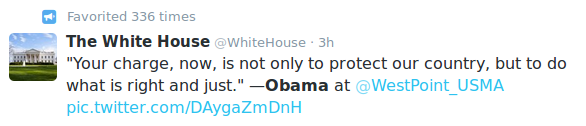
\includegraphics[width=\textwidth]{tweet1} 
    \caption{Typical tweet from Twitter.}
    \label{fig:tweet1}
\end{figure}

%\begin{figure}[htb]
%    \centering
%    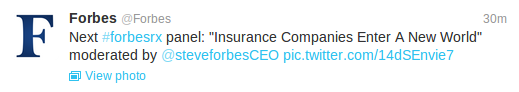
\includegraphics[width=\textwidth]{tweet2} 
%    \caption{The text that shows under the image, image text.}
%    \label{fig:tweet2}
%\end{figure}
%
%\begin{figure}[htb]
%    \centering
%    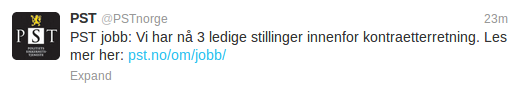
\includegraphics[width=\textwidth]{tweet3} 
%    \caption{The text that shows under the image, image text.}
%    \label{fig:tweet3}
%\end{figure}

\section{Sentiment}\label{previous_work:sentiment}

Opinion mining on the web is not new. In recent years it has
become attractive to traders. 
The use of Twitter and social media is increasing. Both in
business and with private users.
This means a surplus of raw data with
easy access. Companies all over the world has started to use the social
networks to their benefit. The use of information from social media has become
part of the trend, although there are some drawbacks and shortcomings. Noise and
garbage is one of them. Even if you're right 80\% of the time, the last 20\% can
prove devastating. \cite[]{stevenson12:social_media_stock_pickers}

Sentiment broadly refers to a persons state of mind. Based on the opinion the
person will do optimistic or pessimistic choices. A positive mindset leads to
optimistic judgements of future events, and a negative state of mind leads to
pessimistic choices.
\cite[p4]{doukas10:sentiment_and_momentum}

The users may have different roles and intentions in different
communities in the microblogging sphere, \cite[]{java07}. 
A users intentions and its reasons for participation might be a factor in the sentiment analysis.

\subsection{What is Sentiment Analysis}
There are two main categories of approaches to sentiment detection. The first is
to use a classifier. The classifier can use methods such as naive Byes, maximum
entropy or support vector machine \cite[]{Li2013206}. These classifiers are
typical examples where it would be natural to use machine learning of
evolutionary algorithms to increase the classification correctness over time.
The second is use of linguistic resources, such as corpora of negative and
positive words. The developed linguistic resources are used to classify the sentiment of the text \cite[]{Li2013206}.

Li and Li has created a framework for sentiment analysis. The system
consists of four main steps  and is tested with experiments on twitter. 
	First they do topic detection, identifying and extracting the topics
mentioned in the tweet. 
	Secondly opinions are classified. The polarity, how positive a tweets is, of the opinion is decided and
the users impression is captured. 	
	Third. Credibility is assessed. This creates a better summarization of the
expresser's credibility. 
	Fourth, step one, two, and three is aggregated to reflect the true opinion
and point of view.
	Combining the first three steps in the fourth results in a truer reflection of
the expresser's opinion. \cite[]{Li2013206} 

One way of classifying tweets is to use predefined lexicon of positive and
negative words. Consumer confidence and fluctuations of voting polls can be
tracked in this way \cite[]{connor2010}.

The work of \cite[]{diakopoulos2010} describes a methodology for better
understanding of temporal dynamics of sentiment. 
The system uses visual representation to achieve this. 
This is investigated in the reaction to debate video.
	Further \cite[]{diakopoulos2010} detects sentiment pulse and controversial
topics with the help of visualisation and metrics. 
	\cite[]{diakopoulos2010} used crowdsourcing\footnote{Crowdsourcing is the
practice of obtaining needed services, ideas, or content by soliciting
contributions from a large group of people, and especially from an online
community, rather than from traditional employees or suppliers.
\url{http://en.wikipedia.org/wiki/Crowdsourcing}} to classify batches of tweets.
This was accomplished with Amazon Mechanical Turk, a crowdsourcing
site\footnote{Amazon Mechanical Turk (AMT): \url{https://www.mturk.com/mturk/}}.

\cite[]{barbosa10} explores the problem of noise in biased and noisy data. 
They focus on noisy labels and add features to the tweets to increase the
classification properties of the tweets. Objective tweets have very little
sentiment or no sentiment at all. To improve classification, tweets are
classified as objective of subjective. Then the subjective tweets, that have a
sentiment are classified as positive of negative. 

Classification of tweets can be generalised by using features. Features are
small elements of a tweet, such as unigrams, bigrams, or part-of-speech tags.
Bigrams are words consisting of two words, unigrams are words consisting of one
word. An abstract representation of a tweet would be beneficiary to the
classification. In this abstract representation \cite[]{barbosa10} propose to
use characteristics about how tweets are written and meta-information about the
words in tweets.  Meta-features and tweet syntax features that can further improve
classification. Meta-features are information about the tweet, such as location,
language, and number of retweets. Retweets are tweets that are posted again by other users. The tweet syntax features are things such as hashtags, retweet,
reply, links, punctuation and emoticons \cite[]{barbosa10}. 

Challenges with sentiment and twitter is described in another approach by 
\cite[]{becker13}. They explore techniques for contextual polarity
disambiguation and message polarity classification. Constrained and supervised
learning is used to create models for classification. They describe a system
that solves these tasks with the help of polarity lexicons and dependency
parsers. Expanded vocabulary is one of the main aspects of their success, as
they say in their findings: "We hypothesize this performance is largely due to
the expanded vocabulary obtained via unlabeled data and the richer syntactic
context captured with dependency path representations." \cite[]{becker13}

In contrast to \cite[]{becker13}, \cite[]{sperious11} has used distant
supervision and labeled propagation on a graph based data structure. The data
structure represents users with tweets as nodes. And tweets with bigrams,
unigrams, hashtags, etc as subnodes of the tweets. A label propagation approach
rivals a model supervised with in-domain annotated tweets and outperforms the
noisily supervised classifier and a lexicon-based polarity ratio classifier.
\cite[]{sperious11} 

\subsection{Sentiment analysis in Finance}
\cite[p2]{Brown20041} writes the following on over-reaction of investors: 
"\textit{He(Siegel (1992)) concludes that shifts in investor sentiment are correlated
with market returns around the crash. Intuitively, sentiment represents the
expectations of market participants relative to a norm: a bullish (bearish)
investor expects returns to be above (below) average, whatever ‘‘average’’ may
be."}. 
In the light of recent changes in the financial world and the use
of sentiment from social media, the notion that opinions and sentiment of
investors and market actors affect the market is not a new observation.

Use of sentiment can potentially predict changes and trends in the market.
Bad news in an optimistic period creates cognitive dissonance in the small
investors. This impacts the market by slowing down the selling rate of loosing
stocks. \cite[p29]{doukas10:sentiment_and_momentum}
Further we can see that optimistic sentiment has a 2\% monthly average return.
While the investor sentiment is pessimistic we see a drastic reduction in
returns. Down to 0.34\%,\cite[p5]{doukas10:sentiment_and_momentum}.
After optimistic periods it is indicated that the monthly return is reduced to
-0.49\%. On the contrary there is no equivalent change after a pessimistic
period, \cite[p6-7]{doukas10:sentiment_and_momentum}.
Momentum profits are only significant when the sentiment is optimistic,
\cite[p29]{doukas10:sentiment_and_momentum}.

Hope and fear is used by \cite[]{Zhang201155} to decide the movement of the
market. The sentiment is aggregated to be hopeful or fearful. This basically
focuses on positivity and negativity of the sentiment of that particular day.
The daily sentiment is then compared to the market indicators of the same day
to create a prediction of the market. \cite[]{Zhang201155} finds that calm
times give little hope or other emotions. Little turmoil results in few
fluctuations in the market. And opposite, lots of emotions(hope, worry, fear),
gives speed to the market.

\cite[p3]{Brown20041} indicates that the sentiment does not cause subsequent
market returns. For a short-term market timing this is bad news. However
with the changes in social media over the last decade how is the situation
today? With the microblogging sphere of today we can easily see the
correlation of sentiment and the market indicators,
\cite[]{annikajubbega11:twitter_driver_stock_price}. But
does the sentiment cause changes in the market-return?
\cite[p3]{Brown20041} also says that optimism is associated with overvaluation
and subsequent low returns.

\cite[p]{Brown20041} concludes that aggregated sentiment measures has strong
co-movement with changes in the market. He also indicates that sentiment
doesn't appear to be a good trading strategy. This, in the view of
\cite[]{Zhang201155}, indicates a leap in sentiment research and what is possible
with the microblogging of today.

\section{Finance and Trading}\label{previous_work:finance}
%Finance and Trading on and with twitter. 
%\cite[p.2]{annikajubbega11:twitter_driver_stock_price}

The management of assets or liabilities and the management of funds over a
period of time is called Finance. In finance the valuation of assets are time
dependant. The value of an asses is always changing and might not have the same
value five minutes from now. Assets are priced based on expected returns and
risk level. The three sub categories of finance are: personal, corporate and
public \footnote{Wikipedia:\url{http://en.wikipedia.org/wiki/Finance}}. These
categories describes very different parts of the financial world.  

Trading is the action of buying or selling financial instruments.
Financial instruments can be stocks, bonds, derivatives or commodities 
\footnote{Wikipedia:\url{http://en.wikipedia.org/wiki/Trader_(finance)}}.
Trades takes place in markets, stock markets, derivatives markets or commodity
markets.

A new aspect to trading in the last decade has been online trading
\footnote{Wikipedia: \url{https://en.wikipedia.org/wiki/Online_trading}}.
Speed, ease of use, and low costs made the online brokers popular. Many brokers
provide platforms for trade and analysis to select potential investments.  

The tools provided are often some form of technical analysis \footnote{Wikipedia:
\url{http://en.wikipedia.org/wiki/Technical_analysis}}. Technical analysis is
the study of past market data. Mostly volume and price. The purpose of technical
analysis is to forecast the direction of prices.  

Among tools and techniques in technical analysis are charts, market indicators,
and relative strength index. It is also quite common to combine techniques to
acquire better predictions. When looking at put/call ratios, short interest,
implied volatility, and bull/bear indicators of sentiment is also important to take into consideration. 

Technical analysis focus at numeric values, such as volume and price, where fundamental analysis \footnote{Wikipedia:
\url{http://en.wikipedia.org/wiki/Fundamental_analysis}} analyse company health,
financial statements, production rates, earnings, management, and competitive
advantages. Day traders prefer technical analysis over
financial analysis.   

Two principles of technical analysis are, 'History repeats itself', and
'Prices move in trends'. 'History repeats itself' refers to the belief that
traders will do the same actions again and again. Technicians believe that the
repeated behaviour can be recognized as a pattern and be observed on a chart.
'Prices move in trends' is the belief that the price of a commodity will move
directionally over a period of time. Relative highs and relative lows are
indicators of a trend. Consecutive lower highs indicates a downward trend.  

An interesting aspect of trading and finance is the behavioral
one\footnote{Wikipedia:
\url{https://en.wikipedia.org/wiki/Behavioral_finance}}.
Behavioral finance is the field of research that study the effects of
cognitive, social, emotional and psychological factors economic decisions. It
also includes the consequences of resource allocation, market price and
returns. 
%

\section{The Trend}\label{previous_work:trends}
The trend is the general opinion of the masses. As defined by the Free
Dictionary:  
"The direction and momentum of a market, price, economy, or other measure. For
example, if the price of a security is going mainly downward with only a few
gains, it is said to be on a downward trend. Identifying and
predicting trends is important for finding the right moment to buy or sell
securities. Trends are especially important in technical analysis, which
recommends buying at the bottom of a downward trend and selling at the top of an
upward trend."
\footnote{Dictionary description of trend: \url{http://financial-dictionary.thefreedictionary.com/Trend}}

Trends work in much the same way as opinions. People are affected by their
environment all the time. And are often influenced by trends and opinions. When
people are affected by trends they start to move in the same direction as
others. The first group of people that move in the same
direction are called trend setters. They are the people that show others how
the trend works and what this trend is about. 

On twitter we have lots of subcultures that all express themselves on their
specific topic. It can be technology, art, finance, or fashion among others.  
In the sense of twitter we can look at the content of
messages and see if we can find common topics that people talk
about, this being the topic of a subculture or a subspace of twitter. To get
the trend we have to look at the content of the messages in a subspace. Given
that a trend is the combined general opinion of a group. We can analyse the
group and see if we can find certain topics or areas of interest that aggregates
to a trend.  

Stock market prediction
\footnote{Wikipedia: \url{http://en.wikipedia.org/wiki/Stock_market_prediction}}
is the act of trying to predict or determine the future
value of a stock. A way to do this is to look for trends in the data. The trend
is a tendency of movement in a particular direction for a financial market.

There are three categories of trends in finance. Primary, secondary and secular
trends. Where primary trends have a medium time frame, secondary have a short
time frame, and secular has long time frames \footnote{Wikipedia:
\url{http://en.wikipedia.org/wiki/Market_trend}}. Bull market and bear market
are terms that, respectively, describe upward and downward market trends. 
Trends are often found by using technical analysis.  

Secular trends are trends that last between 5 and 25 years. A secular bull
market consists of many larger bull markets and many smaller bear markets.
Primary trends last a year or more. We can also observe market tops and
bottoms here. These are trend reversal points. Secondary trends has a
duration of a few weeks or months. The secondary market trend is change in
price direction within a primary trend. The small changes are often called
market corrections. The short term correction is often between 5 and 20 percent.

When looking for usage of twitter trends, we find little to confirm research in
this area. 
%
 % why / what 
\chapter{Data, retrieval and structure}
% The data. What used, how and why. Acquired data how and from where. 

This section describes the data sources, methods for acquisition, and the
structure of the used data. \ref{data:tweets} describes twitter and the mined
tweets. \ref{data:dictionaries} describe the different lists of words used in
the classification process. And last the finance data is described in
\ref{data:finance}.

For each section the structure, characteristics, metadata and usage are
described. 

#TODO chapter outline
%

% The section about twitter and tweets 
\section{Tweets}\label{data:tweets}
A tweet is a massage posted on twitter. The message can be up to 140 characters
long and in many ways it resembles the well known
SMS\footnote{Wikipedia on Short Messaging Service:\url{https://en.wikipedia.org/wiki/Short_Message_Service}}.

Tweets are posted to the users profile. When other people posts a previously
posted tweet again it is called a retweet.

All users can follow other users on Twitter. Tweets from users you follow will
appear in you stream of tweets on the main page of twitter.
%

\subsection{Tweet Structure}
\paragraph{Structure}
\hspace{0pt}\\
There are a lot of metedata in the tweets. In fact most of the data in a tweet
object is metadata. 

The data we acquire from Twitter is in the JSON data format. JSON or \textit{JavaScript
Object Notation} is an open standard format that uses human-readable text to
transmit data objects consisting of attribute–value
pairs\footnote{Wikipedia on JSON:\url{https://en.wikipedia.org/wiki/Json}}.


A positive thing about the JSON data format is that we can directly evaluate it
in python. By using literal evaluation in python the tweet object is
interpreted as a dict. This makes the use of a tweet easy.  

For an example of the data structure of a tweet, see appendix:
\ref{appendix:tweetStructure}.

\paragraph{Content}
\hspace{0pt}\\
A tweet is an astonishing compilation of data about who, where and when a tweet
was posted.

As for the content we have the text, the message itself. With the content we
have fields for all the links, all the emoticons, and all hashtags that are
present in a tweet. 

Every tweet is posted by a user. All the data of a user is also present for
each tweet. Here we have data on follower count, profile images, friend count,
time zone, and many other profile related items. 

For the sharing of a single tweet we have data fields such as favorite\_count
and user\_mentions. We also have favorited, retweet\_count. 

In addition we have the location of a given tweet. Where the tweet was posted,
the name of the place, the coordinates of the tweet, the country, and the id of
this place. 

See all the different metadata types in appendix: \ref{appendix:tweetStructure}.
%

% data acquisition
\subsection{Twitter API}
The twitter API is a convenient way for lots of people to access data from
twitter. Tweets, streams, timelines, profiles and more are available through
the api. 

To provide easy easy access and conformity to industry standards, the api
provides data in the JSON format. 

While the api does not give access to 100\% of the data from twitter, it gives
a good representation of the tweets from the last 7 days.
%

\paragraph{Setup}
\hspace{0pt}\\
To get access to the api there are a few requirements. You have to have a
twitter account. You have to register the application you are going to use the
api with, thereby getting authentication keys. Then you have to used the keys
authenticate with twitter before you access the api. 

For a simple guide to this we have
\url{http://datascienceandprogramming.wordpress.com/2013/05/14/twitter-api/} as
a good example.

The 4 authentication tokens you get from Twitter, app\_key, app\_secret, oauth\_token,a nd
oauth\_token\_secret, is used with the Twython
library\footnote{\url{https://pypi.python.org/pypi/twython/}} as described
below.

The simplest example of use of the api and the twython library can be described
as follows:
\begin{itemize}
	\item Authenticate towards twitter.
	\item Execute search query on twitter.
	\item Print ID's of all retrieved tweets.
\end{itemize} 

The code of the example is as follows:
\begin{listing}
\begin{verbatim}
twitter = Twython(APP_KEY, APP_SECRET, OAUTH_TOKEN, OAUTH_TOKEN_SECRET)
results = twitter.search(q='Search query', count='15')

for status in results['statuses']:
    print status['id']
\end{verbatim}
\end{listing}

For more advanced use we have generators, and lots of parameters and api
endpoints to use. Endpoints and search parameters will be described under
section \ref{data:twitter:endpoints}, \textit{API endpoints options}. 
The twyhon framework and its advanced usage can be explored more in the code and
in the documentation of the framework
\footnote{\url{https://twython.readthedocs.org/en/latest/usage/advanced_usage.html}}.
%

\paragraph{Restrictions}
\hspace{0pt}\\
#TODO API restrictions\\
request restrictions.
%

\paragraph{API endpoint options}\label{data:twitter:endpoints}
\hspace{0pt}\\
This is a list of the most useful endpoints and those used in the thesis.
\begin{itemize}
\item[q] A UTF-8, URL-encoded search query of 1,000 characters maximum, including
operators. Queries may additionally be limited by complexity.

\item[count] The amount of tweets acquired in each request. Standard = 15, max
= 100. 

\end{itemize}
%

\paragraph{Searching}
\hspace{0pt}\\

%

\paragraph{Mining optimization}
\hspace{0pt}\\
#TODO -rt, searching vs generator\\ 
%

\paragraph{Caveats}
\hspace{0pt}\\
Please note that Twitter's search service and, by extension, the Search API is
not meant to be an exhaustive source of Tweets. Not all Tweets will be indexed
or made available via the search interface.
%

\subsection{Tweet sets}
#TODO manual classification\\
#TODO search terms\\
#TODO limitations\\
%

\subsection{Biased Data}
#TODO write this section\\
Due to the necessity of a search term in the query, we only get tweets that are
related to the given terms.

Further more the datasets of manually labeled tweets are biased based on my
personal opinion and state of mind in the moment of classification.  

\subsection{Trend Data}
#TODO Briefly describe the mining and API shortcomings for this particular
use.\\
#TODO describe the trend search terms: '\_search-terms'\\
#TODO write shortcomings of the search terms. \\
#TODO Describe the tweet data sets and sorting. \\ 

\subsection{Problems, Shortcomings, and Possible Improvements}
The potential problems and shortcomings of the data. 

#TODO retweets.\\ 
#TODO search terms.\\
#TODO finance vs not finance.\\

% describing the dictionaries used in the classification of tweets. 
\section{Dictionaries}\label{data:dictionaries}
#TODO introduction to dictionaries, of corpus whatever the name. \\
#TODO the purpose of the dictionary\\
#TODO use of the dictionaries. \\
%

\subsection{Downloaded Dictionaries}
#TODO describe the distinctions of dl dict

\paragraph{Obama}
\hspace{0pt}\\
#TODO describe obama dictionary.\\ 

\paragraph{Loughran & McDonald}
\hspace{0pt}\\
#TODO describe this dictionary
Tim Loughran and Bill McDonald has a set of dictionaries available from the
websites of University of Notre Dame \footnote{#TODO fiks tekst: nd.edu:
\url{http://www3.nd.edu/~mcdonald/Word_Lists.html}}. 

List of Dictionaries:
\begin{itemize}
    \item negative words
General list of negative words. No particular category. Used for basic   
    \item positive words
This dictionary contains a small set of positive words. There are no general
category for the words. The words are not directly related to finance. 
    \item Uncertainty words
    \item litigious words
    \item modal words strong
    \item modal words weak
\end{itemize}
%

\subsection{Compiled Dictionaries}
The compiled dictionaries are based on two manually labeled tweet sets. My own,
the kiro dataset, and the obama tweet set.
 
#TODO ref the used datasets.\\ 

Details about the process of manually classifying tweets can be found in section
\ref{sentiment:manual_classification}.

#TODO describe the dictionary compilation.\\


List of dictionaries:

#TODO describe the different dictionaries\\ 
\begin{itemize}
    \item Obama original, Monogram 
	\subitem description

    \item LoughranMcDonald, Monogram 
	\subitem description

    \item Obama original and LoughranMcDonald, Monogram, combined
	\subitem description

    \item Kiro, Monogram, self compiled 
	\subitem description

    \item Obama, Monogram, self compiled 
	\subitem description

    \item Kiro, Bigram, self compiled 
	\subitem description

    \item Obama, Bigram, self compiled 
	\subitem description

    \item Kiro, Trigram, self compiled 
	\subitem description

    \item Obama, Trigram, self compiled 
	\subitem description
	\label{data:dictionary_list}
\end{itemize}
%

\subsection{Error analysis, removal of duplicate words}
When creating the different dictionaries we remove duplicates from the positive
and negative dictionary set. Words that are present in both the positive and
negative dictionary is removed. By doing this we remove words that has no
significance in the classification. But we also risk removing words with
significance.

When looking at the duplicate words from the monogram dictionary based on the
kiro dataset we found some errors.
As a selection of words found, we have \textit{dangerous, bad, go, inc, let, up, or, need, good, if, no, are, and, of, on, the,
is, as}.
Here we can see that the words \textit{good} and \textit{bad} are represented.
Which is not good. By removing the words from the dictionaries we have removed
significant words in further classification, thus reducing correctness of the
algorithm. This is one of the drawbacks of the monogram dictionaries.

When looking at the removed duplicate words for bigram and trigrams we found no
indication of the same problem. As the uniqueness of bigrams and trigrams are a
lot greater we end up with very few duplicates and only duplicates that has no
significance to the over all classification. Although we might have other
unknown problems.  

Most stop words and other insignificant words are removed with the removal of
duplicate words. The same thing cannot be said about the bigram and trigram
dictionaries. There we have no stop words present in themselves, but they are
frequently part of other terms. For further improvements of classification with
word counting and dictionary quality we should remove
stop words, such as \textit{as, is, on, off, and, or} etc, from the
tweet/sentence before creating bi- and trigrams.     
%

% The financial data used in the thesis. 
\section{Finance Data}\label{data:finance}
#TODO obtaining the data(potential mining operations)
#TODO about the dataset, csv
#TODO potential problems 
%

 % how

\chapter{Sentiment Analysis}
This section describes the experiments done. High level description and
execution of experiments. Detailed execution and technical details in appendix. 

\section{What we use the sentiment for in this thesis.}
\section{Getting the sentiment}
\subsection{Techniques}
\subsection{- of a Tweet}
\section{Sentiment trend}
\section{Experiments}
% todo figure out what experiments are smart to do. 

* Experiment with the time frame of the prediction of the trend. 
	* Typically the variation of time. What's the longest into the future that
we can predict the trend?
* 

\subsection{Recreate sentiment classification with lexicons of positive and
negative words.}

A basic approach to classification is to count words. Positive and negative
words. To do this it is necessary have dictionaries to provide the
classification of simple words. Section:\ref{sec:dict} describes the
dictionaries used. Some of them are quite simple, while others are more
extensive. 

The polarity of a given tweet is based on the difference in the amount of
positive verses negative words. 

Todo: run an experiment with 100+ tweets to see to what extent the
classification works. Further this has to be compared to a control set, of
manually classified tweets.  

\subsection{Features addition to tweets.}
\subsection{labeled graph propagation.}
\subsection{Combination of the three above}
\subsection{Trend creation}
\subsection{comparrison}
 % how

\chapter{Trending}
#TODO outline this chapter. 
%

\section{The trend is your friend}
#TODO why do we want a trend?
What is a trend. How do I define it? How do I use it in this context? And how
does it work? 
%

\section{Trends on Twitter}
#TODO trends on twitter already.
#TODO what the trends are and what to use them for. 
#TODO how we created the trend graph
#TODO Our own trend. compiled
 
How we can find trends on twitter and how we can use them.
% 

\section{Trending in Finance}
#TODO how can we see trends in finance if any at all?
#TODO hoped use of the trend compilation. 

How trends are in finance. How we find them and what we use them for. 
%

\section{Comparing the trend and the moving average}
#TODO comparing the twitter trend, compiled trend and finance input. 
#TODO any correlations among the trends?
#TODO what we get out of the trend we have created
#TODO if the trend created have any strong points?
#TODO What went wrong?
#TODO lessons learned of the trend? 
 
Comparing a found trend on twitter with a found trend in finance. Are there
correlations?   
%
 % how
\chapter{Experiments}\label{experiments}
This chapter aims to test methods described in earlier chapters. We describe
setup and context for the experiments as well as the used data.

The experiments described in this chapter are the following: Dictionary
compilation, \ref{experiments:dictionaries}. The word count classification, bag
of words method, \ref{experiments:word_count_classification}. Threshold
variation in section \ref{experiments:threshold}. Kernel choice for the SVM
classifier is described in section \ref{experiments:svm_kernel}. The
testing of classifiers is found in section \ref{experiments:calssifiers}. And
trend aggregation in section \ref{experiments:trend}.

\section{Dictionary Compilation}\label{experiments:dictionaries}
Section \ref{data:dictionaries} describe dictionaries and what they are used
for. The dictionaries are compiled from manually labeled tweets.
This section describes how the dictionaries are tested. 

The dictionaries were created for the word count classification, 
as a step in the sentiment classification research.
To find which dictionaries performed well, or not, we tested them
with two data sets, the Kiro dataset and the Obama dataset. 

The quality of the dictionary is tested by removing duplicate words. This gives
an indication of the correctness of the dictionary. 
Words that are present in both the positive and
negative dictionary are removed. By doing this we remove words that has no
significance in the classification. But we also risk removing words with a 
clear sentiment. The code is described in appendix
\ref{code:remove_duplicate_words} on page \pageref{code:remove_duplicate_words}.

This experiment enlightens part of research question 1,
how we can find the sentiment of a tweet.

The quality of the dictionary is given by the number of correct classifications
it gives. The results of classification with each dictionary is described in
tabled \ref{tbl:classification_comparison}, on page
\pageref{tbl:classification_comparison}. 

Results from the testing of dictionaries are closely linked to the word count
classification in section \ref{experiments:word_count_classification} and shown in
table \ref{tbl:sentiment_word_count_results} on page
\pageref{tbl:sentiment_word_count_results}.
%

\section{Word Count Classification}\label{experiments:word_count_classification}
The background for the experiment and it's purpose is described in section
\ref{sentiment:classification}. This experiment used the technique described in
section \ref{sentiment:word_count_classification}, the word count method of
classifying a tweets sentiment.  

The main goal of this experiment is to determine the sentiment
of a tweet, section \ref{introduction:rq1}. And how Twitter can be used, indirectly, to
aggregate a trend, section \ref{introduction:rq2}.
The method looks at the number of positive and negative words and use
that to decide the sentiment we have.

Both datasets are classified with all the dictionaries. This
gives the accuracy for all dictionaries for the two datasets, and indicates the
efficiency of the word count classification. 

The accuracy of the classification is determined by looking at the number of
tweets that were classified correctly. The accuracy is the percentage of
correctly classified tweets.  

The code for calculating the sentiment is as follows. It is also described in
appendix \ref{code:word_count_classification}, on page
\pageref{code:word_count_classification}.
\begin{python}
positivity = positive_words_count / total_number_words
negativity = negative_words_count / total_number_words

polarity = positivity - negativity

if polarity > 0:
    tweet is positive
else:
    tweet is negative
\end{python}

The results of the classification can be found in section
\ref{results:word_count_classification} on page
\pageref{results:word_count_classification}.
%

\subsection{Threshold Variation}\label{experiments:threshold}
In section \ref{sentiment:threshold} the description and purpose of the
threshold variation is described. The threshold gives a degree of positivity. Or
rather how many more positive words than negative words we need to call the
tweet positive.  

By varying the threshold we hoped to find an optimal point where we could
separate tweets based on polarity. From the threshold graphs in figure
\ref{fig:threshold_graphs}, page \pageref{fig:threshold_graphs}, we can see no
clear distinction of one value being better than others.

What is done is that the word count classification is run multiple
times with varying threshold values. Values between -0.9 and 0.9. This gives a
distribution of results which is plotted in graph
\ref{fig:average_threshold_accuracy} on page
\pageref{fig:average_threshold_accuracy}.
The results gives an indication of what threshold is best for word counting. 

The results of the threshold variation is described in section
\ref{results:threshold}, on page \pageref{results:threshold}. And in table
\ref{tbl:average_threshold_accuracy} on page
\pageref{tbl:average_threshold_accuracy}.
%

\section{Using Classifiers}\label{experiments:calssifiers}
The two datasets was tested with the two trained classifiers.
This was done to find the best classifier.
We found the best classifier by comparing the results of the two trained
classifiers and the word count classification. 

Description of the comparison, on a conceptual level, is described in section
\ref{sentiment:comparison_results}. 
The experiment takes inspiration from concepts described in section
\ref{previous_work:sentiment}.

The research questions to be enlightened by the experiment is the trend
aggregation(RQ1) in section \ref{introduction:rq1} and the sentiment
classification(RQ2) in section \ref{introduction:rq2}.
%

\subsection{SVM}\label{experiments:svm_classification}

\paragraph{Choice of SVM Kernel}\label{experiments:svm_kernel}
\hspace{0pt}\\
In extension of section \ref{sentiment:svm_classification} all the SVM kernels were
tested.
While testing which kernel was best we used the Kiro dataset for training, and
the Kiro monogram dictionary for feature extraction.

Using the self compile monogram dictionaries and all the different SVM kernels
we get the results described in table \ref{tbl:svm_classifier_kernel_test}, page
\pageref{tbl:svm_classifier_kernel_test}.

\begin{table}
\centering
\label{tbl:svm_classifier_kernel_test}
\caption{SVM kernel test results table}
\begin{tabular}{ l r r c }
Kernel & Failed & Correct & Accuracy \\
\hline
LinearSVC & 7 & 990 & 0.9930 \\
NuSVC & 29 & 968 & 0.9709 \\
NuSVR & 422 & 575 & 0.5767 \\
OneClassSVM & 575 & 422 & 0.4233 \\
SVC & 422 & 575 & 0.5767 \\
SVR & 422 & 575 & 0.5767 \\
\end{tabular}
\end{table}

\paragraph{SVM Classification}
\hspace{0pt}\\
Results from testing SVM with different dictionaries are described in table
\ref{tbl:svm_classifier_results} on page
\pageref{tbl:svm_classifier_results}.

\begin{table}
\centering
\label{tbl:svm_classifier_results}
\caption{SVM classifier results table}
\begin{tabular}{ l l r r c }
Dataset & Type & Failed & Correct & Accuracy \\
\hline
Kiro & Monogram & 7 & 990 & 0.9930 \\
Kiro & Bigram & 422 & 575 & 0.5767 \\
Obama & Monogram & 35 & 1330 & 0.9744 \\
Obama & Bigram & 507 & 858 & 0.6286 \\
\end{tabular}
\end{table}

\subsection{Naive Bayes}\label{experiments:naive_bayes_classification}
\hspace{0pt}\\
Results from testing Naive Bayes with different dictionaries are described in
table \ref{tbl:naive_bayes_classification_results} on page
\pageref{tbl:naive_bayes_classification_results}.

\begin{table}
\centering
\label{tbl:naive_bayes_classification_results}
\caption{Naive Bayes classifier results table}
\begin{tabular}{ l l r r c }
Dataset & Type & Failed & Correct & Accuracy \\ 
\hline 
Kiro & Monogram & 29 & 968 & 0.9709 \\
Kiro & Bigram & 29 & 968 & 0.9709 \\
Obama & Monogram & 59 & 1306 & 0.9568 \\
Obama & Bigram & 59 & 1306 & 0.9568 \\
\end{tabular}
\end{table}
%

\section{Trend Aggregation}\label{experiments:trend}
Section \ref{trend:compared} describes the
conceptual parts of the trend comparison. This is the basis for the results of
this experiment. 

This experiment aims to test the relevance of positive and negative tweets in
correlation with change in finance. There are two parts to this experiment. The
finance part, and the twitter part. Can twitter be used to create a trend,
\ref{introduction:rq2}. And how can we compare this to a finance trend,
\ref{introduction:rq3}.

In the execution of the experiment the methods described in chapter \ref{trend}
has been used. More specifically the trend aggregation under 'trends on
twitter', section
\ref{trend:trends_on_twitter}. And the finance trend aggregation in
section \ref{trend:trends_in_finance}.

The tweet data used is described in section \ref{data:trend_data}, on page
\pageref{data:trend_data}. And the finance data is described in section
\ref{data:finance}, page \pageref{data:finance}.

The results of the experiment is discussed in section \ref{results:trend}. 
%
 % what
\chapter{Results and Discussion}\label{results}
%All our results are in ones and zeroes. 
%And further we discuss why there are only zeroes. And how that affects the
%outcome and future endeavors for the pirates we are. 

The results of our research and the following discussion of them happen here.
We touch the main parts of the thesis. The data sources, section
\ref{results:data_sources}. Dictionaries, section \ref{results:dictionaries}. Classification of sentiment in section
\ref{results:classification}. And the trend in section \ref{results:trend}.
Last we have a general discussion about the results. 
%

\section{Data Source}\label{results:data_sources}
Twitter as a data source proved to be OK. It was quite easy to obtain data. But
increasingly difficult to get good amounts of data and unbiased data. All the
initial data have some restriction to search words or other limits. In total we
should have mined a lot more data and manually classified more of it. 

As far as the dictionaries go they work well. We have different results for
different dictionaries and different datasets, but all in all the way to
compile datasets work good. The dictionaries depend on the manually classified
tweets, so a lot of the potential improvement lies there. Although we can
improve the dictionaries by removing stop words and other words we know have no
clear positive of negative sentiment. 

In research question 1, \ref{introduction:rq1}, we asked what knowledge we can
extract from tweets to find a sentiment. The dictionaries are a good way to
compose sentiment from the different words in the manually labeled tweets.

Research question 3, \ref{introduction:rq3}, asks if Twitter has been useful in
comparison with technical analysis. To some  extent it has. We have mined and
classified many tweets in the hope that the aggregated trend would show
likeness to plots of technical analysis. The data from Twitter that has been
used to acquire positive and negative tweets for the trend aggregation. And has
also provided useful insight into the use of the Twitter API. 
%

\section{Dictionaries}\label{results:dictionaries}
As for the use of the dictionaries in association with the trend and research
question 3, \ref{introduction:rq3}, we use the dictionaries for feature
extraction in the classifiers. Besides the use in classifiers the dictionaries
have no other practical uses in this thesis in relation to sentiment.

\paragraph{Error analysis}
\hspace{0pt}\\
When looking at the duplicate words from the monogram dictionary based on the
kiro dataset we found some errors.
As a selection of words found, we have \textit{dangerous, bad, go, inc, let, up,
or, need, good, if, no, are, and, of, on, the,
is, as}.
Here we can see that the words \textit{good} and \textit{bad} are represented.
Which is not good. By removing the words from the dictionaries we have removed
significant words in further classification, thus reducing correctness of the
algorithm. This is one of the drawbacks of the monogram dictionaries.

When looking at the removed duplicate words for bigram and trigrams we found no
indication of the same problem. As the uniqueness of bigrams and trigrams are a
lot greater we end up with very few duplicates and only duplicates that has no
significance to the over all classification. Although we might have other
unknown problems.

Most stop words and other insignificant words are removed with the removal of
duplicate words. The same thing cannot be said about the bigram and trigram
dictionaries. There we have no stop words present in themselves, but they are
frequently part of other terms. For further improvements of classification with
word counting and dictionary quality we should remove
stop words, such as \textit{as, is, on, off, and, or} etc, from the
tweet/sentence before creating bi- and trigrams.
%

\section{Classification}\label{results:classification}
Manual labeling is a bit of a challenge to keep unbiased. The whole
classification process is based on a persons opinion, which makes the results
somewhat biased. To eliminate this error we should have multiple people do the
manual classification and combine the results.  

Word counting works to some extent. But presents varied results based on the
dataset and the dictionary used. Again this comes down to the dataset and the
dictionaries created. Also the way we separate tweets from each other with a
threshold can be improved. All in all word counting works, but it is not very
good. 

Classifiers  improve the classification quite a bit. With the svm classifier we
get around 98 percent correct classification on both data sets. Which is good.

The uncertainties lie in the biased, or potentially biased, data. We do not
know if the data in itself is fully representable for the content on twitter.
Neither do we know if the manual classification is completely correct. 

In total we gained some knowledge about dictionaries and their effect on
classification. And we can confirm that classifiers work better than word
counting.  

We tested two ways of finding the sentiment of a tweet. The bag of words method
described in section \ref{sentiment:word_count_classification}, and the
classifier way with the SVM and Naive Bayes classifiers,
\ref{sentiment:classification}.

Research question 2, \ref{introduction:rq2}, the question of trend aggregation,
the classification was useful. The sentiment worked to some extent. We do not
know how well. And we have to look into the part of credibility in future work.   
%

\subsection{Word Count Classification}\label{results:word_count_classification}
The results from the word count classification can be plotted in the tabled
\ref{tbl:sentiment_word_count_results} and in the graph
\ref{tbl:sentiment_word_count_results}.

\begin{table}
\centering
\label{tbl:sentiment_word_count_results}
\caption{Word Count classification results table}
\begin{tabular}{ r p{6cm} r r c }
id & Dictionary & Failed & Correct & Accuracy \\
& -- Kiro compiled dataset -- & a & b & b/(a+b) \\
\hline
1 & Monogram, Obama & 578 & 419 & 0.4203 \\
2 & Monogram LoughranMcDonald & 491 & 506 & 0.5075 \\
3 & Monogram, combined Obama and LoughranMcDonald & 416 & 581 & 0.5827 \\
4 & Kiro, Monogram, self compiled & 115 & 882 & 0.8847 \\
5 & Kiro, Bigram, self compiled & 17 & 980 & 0.9829 \\
6 & Kiro, Trigram, self compiled & 18 & 979 & 0.9819 \\
7 & Obama, Monogram, self compiled & 567 & 430 & 0.4313 \\
8 & Obama Bigram, self compiled & 534 & 463 & 0.4644 \\
9 & Obama Trigram, self compiled & 567 & 430 & 0.4313 \\
& -- Obama tweet set -- & a & b & b/(a+b) \\
\hline
10 & Monogram, Obama & 855 & 510 & 0.3736 \\
11 & Monogram LoughranMcDonald & 508 & 857 & 0.6278 \\
12 & Monogram, combined Obama and LoughranMcDonald & 544 & 821 & 0.6015 \\
13 & Kiro, Monogram, self compiled & 632 & 733 & 0.5370 \\
14 & Kiro, Bigram, self compiled & 521 & 844 & 0.6183 \\
15 & Kiro, Trigram, self compiled & 498 & 867 & 0.6352 \\
16 & Obama, Monogram, self compiled & 493 & 872 & 0.6388 \\
17 & Obama Bigram, self compiled & 37 & 1328 & 0.9729 \\
18 & Obama Trigram, self compiled & 39 & 1326 & 0.9714 \\
\end{tabular}
\end{table}

5, 6, 17, 18 are the dictionaries with best accuracy. Which is to be expected
for the classification of the dataset the dictionary was created from.

But more interestingly, if we take the dictionaries created form one dataset,
and look at the results of the classification on the other dataset. We compare
7, 8, 9 with each other and 13, 14, 15 with each other. Then we can see that
the bigram and trigram dictionaries perform overall better than the monogram
dictionaries.

Further we see indications that the quality of the dictionary plays an
important role. The LoguhranMcDonald monogram dictionary performs quite good
with both datasets. Even on par with the compiled dictionaries on opposite
dataset. This indicates that a well crafted dictionary can perform as well
as compiled dictionaries.

\begin{figure}[htb]
    \centering
    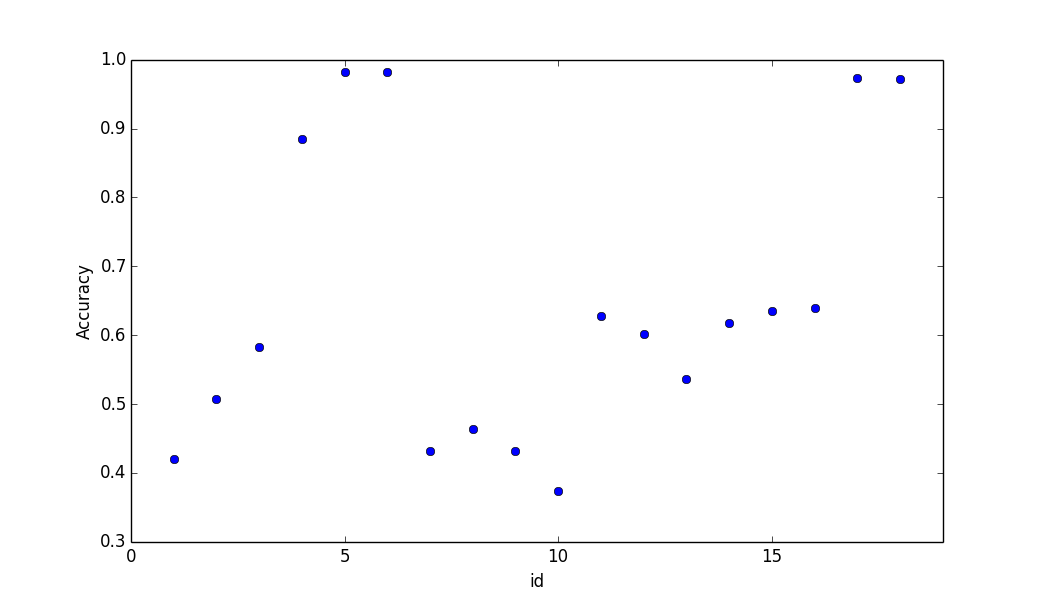
\includegraphics[width=\textwidth]{dictionary_accyracy.png}
    \label{fig:dictionary_accyracy}
    \caption{Dictionary Accuracy plot}
The graph shows the plotted accuracies from the word count
classification. The ids represents the ids from the table above,
\ref{tbl:sentiment_word_count_results}
\end{figure}

When comparing the results from one dataset to the other we can see indications
of how the content of the dataset also plays a huge role in the results. Some
tweets are more difficult to classify then others.

There are a lot of improvements that could be done.
The word count classification is merely a convenient way to say something about
the dictionaries used. We should expand our knowledge toward the quality of the
dictionaries. And look for ways to eliminate terms that are neither positive or
negative. 

\subsection{Threshold Variation}\label{results:threshold}
Further we found the best average threshold value to be 0.1.
From the table under we have the threshold value, and the average
classification accuracy among the 18 entries for each threshold value.

\begin{table}
\centering
\label{tbl:average_threshold_accuracy}
\caption{Average threshold accuracy table.}
\begin{tabular}{ c c c c }
Threshold & Accuracy & Threshold & Accuracy \\
\hline
- & - & 0.0 & 0.6479 \\
-0.1 & 0.6316 & 0.1 & 0.6516 \\
-0.2 & 0.6161 & 0.2 & 0.6511 \\
-0.3 & 0.6059 & 0.3 & 0.6430 \\
-0.4 & 0.5988 & 0.4 & 0.6305 \\
-0.5 & 0.5888 & 0.5 & 0.6122 \\
-0.6 & 0.5711 & 0.6 & 0.5934 \\
-0.7 & 0.5423 & 0.7 & 0.5712 \\
-0.8 & 0.5083 & 0.8 & 0.5457 \\
-0.9 & 0.4881 & 0.9 & 0.5307 \\
\end{tabular}
\end{table}

\begin{figure}[htb]
    \centering
    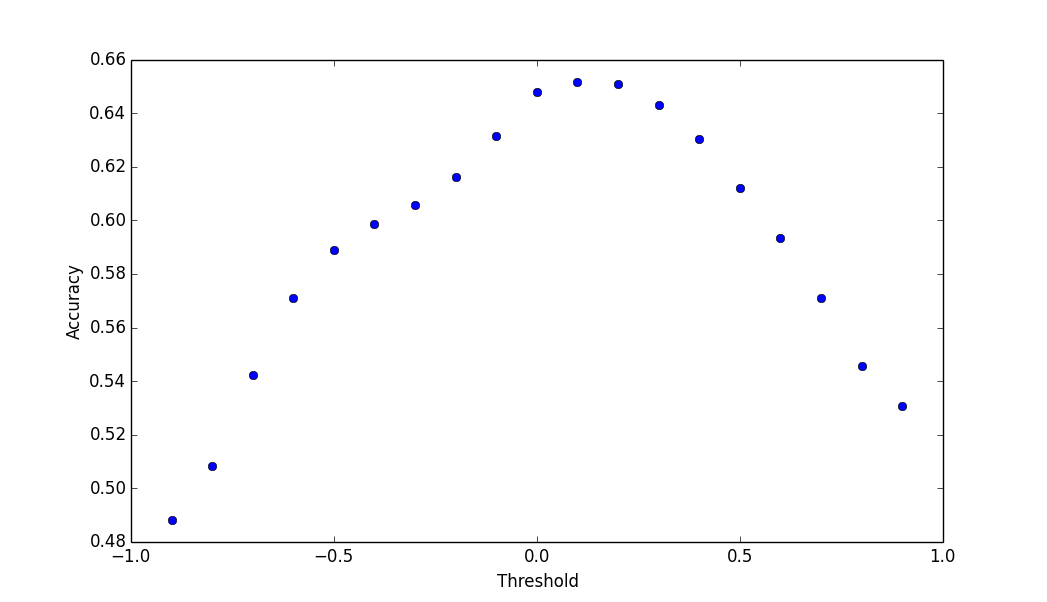
\includegraphics[width=\textwidth]{average_threshold_accuracy.png}
    \label{fig:average_threshold_accuracy}
    \caption{Average threshold accuracy}
Graph plots of the 'Average threshold accuracy' table.
\end{figure}

In figure \ref{fig:threshold_graphs} we list the results of the experimentation
with the threshold. Table \ref{tbl:dictionary_to_threshold} lists the
dictionaries and dataset used for which graphs in figure
\ref{fig:threshold_graphs}.
'kiro dataset' and 'obama dataset' columns tells which dataset that was
classified in which graph.

\begin{table}
\centering
\label{tbl:dictionary_to_threshold}
\caption{Dictionary to threshold graph plot table}
\begin{tabular}{ l c c }
Dictionary name and description & kiro dataset & Obama dataset \\
\hline
Obama original, Monogram & 1 & 10 \\
LoughranMcDonald, Monogram & 2 & 11 \\
Combined Obama original and \\ LoughranMcDonald, Monogram & 3 & 12 \\
Kiro, Monogram, self compiled & 4 & 13 \\
Obama, Monogram, self compiled & 5 & 14 \\
Kiro, Bigram, self compiled & 6 & 15 \\
Obama, Bigram, self compiled & 7 & 16 \\
Kiro, Trigram, self compiled & 8 & 17 \\
Obama, Trigram, self compiled & 9 & 18 \\
\end{tabular}
\end{table}

\begin{figure}[htb]
    \centering
    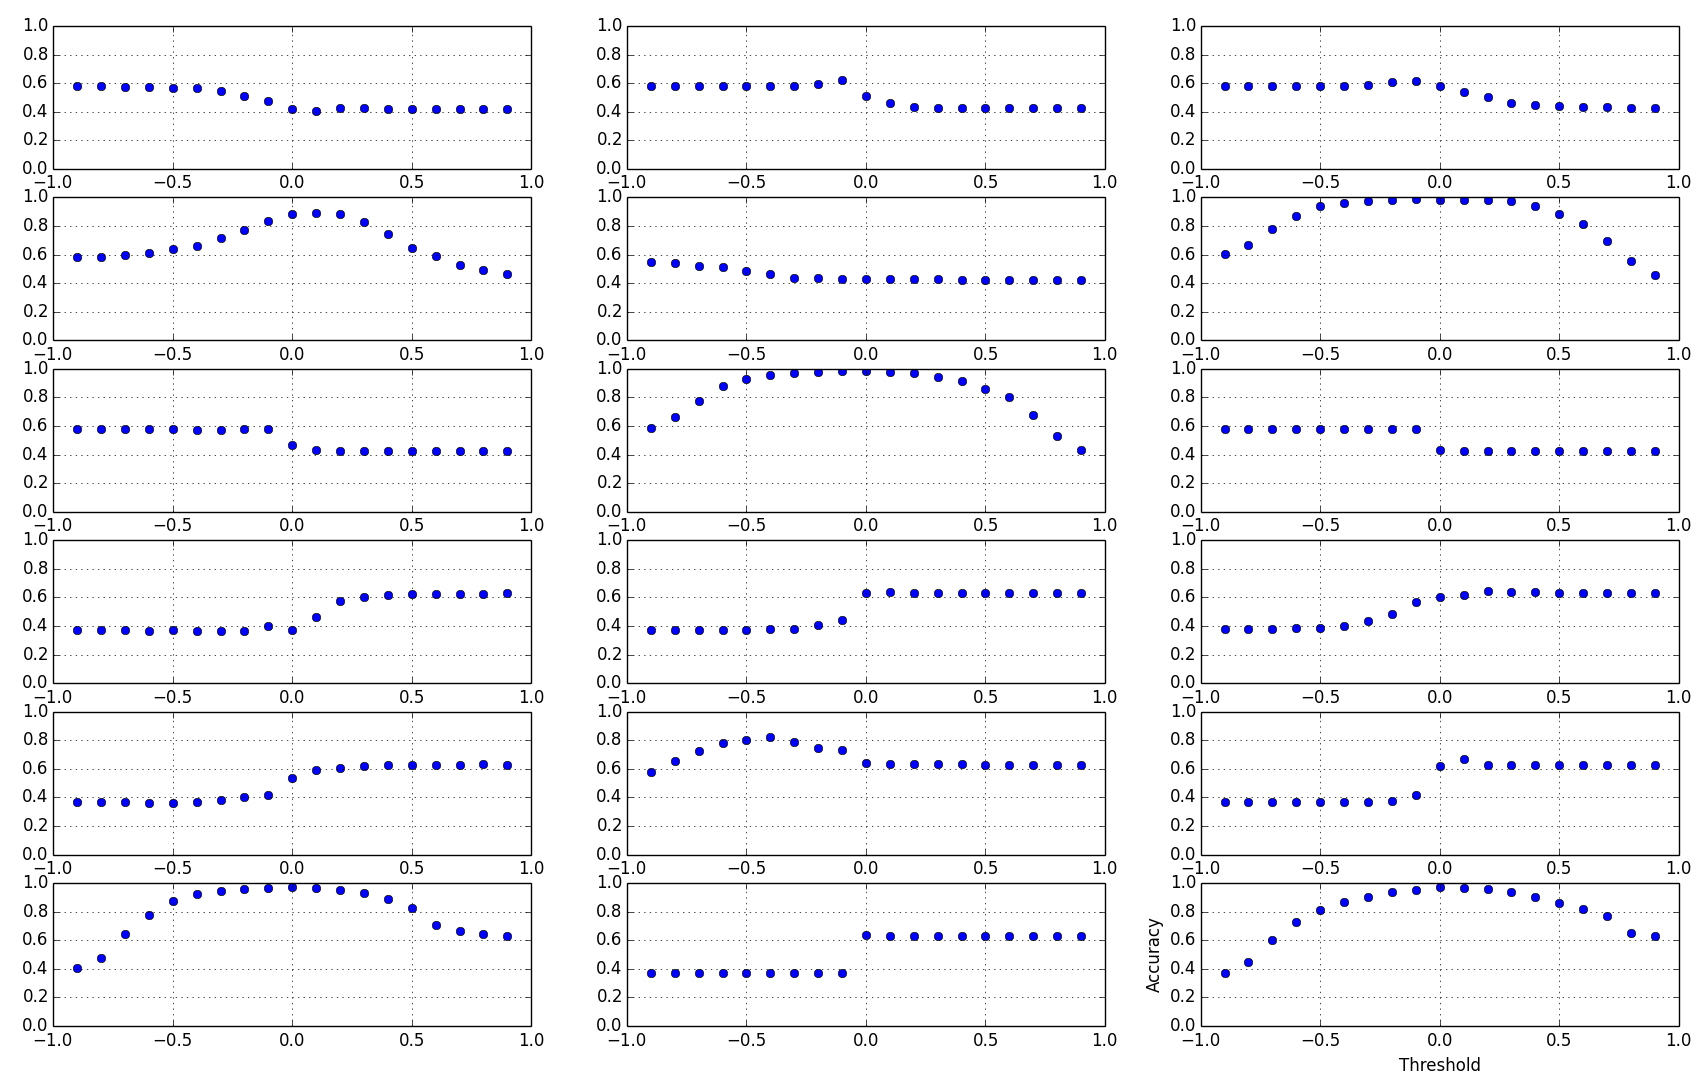
\includegraphics[width=\textwidth]{threshold_graphs.png}
    \label{fig:threshold_graphs}
    \caption{Threshold variation accuracy plot}
The graphs plot the different variations of threshold. Counting is
columns first; top left is 1, top mid is 7, top right is 13.
\end{figure}

\subsection{Using Classifiers}
Not surprisingly the classifiers have better results than the bag of words
method of classification. Further the SVM classifier with the LinearSVC kernel
module performed best. Naive Bayes classifier was nearly as good. This answers
part of research question 1, \ref{introduction:rq1}.

\paragraph{SVM}\label{results:svm_classification}
\hspace{0pt}\\
From results of the experiment, \ref{experiments:svm_classification}, we can draw
some conclusions. The monogram dictionary performed
better than the bigram dictionary. Probably due to the number of features we
can extract from each tweet. Also classifiers are more accurate than the word
count classification method.

\paragraph{Naive Bayes}\label{results:naive_bayes_classification}
\hspace{0pt}\\
As we can see from the experiment,
\ref{experiments:naive_bayes_classification}, the different dictionaries makes
no difference for the Naive Bayes classifier. But if we compare the classifier
with the results from the word count classification we can clearly see
improvement. 

\subsection{Comparison}\label{results:comparison}
In the following table, \ref{tbl:classification_comparison}, we highlight the
results from the different classifications. We list the most noteworthy results
from our experiments and compare them.

\begin{table}
\centering
\label{tbl:classification_comparison}
\caption{Comparison of classifiers table}
\begin{tabular}{ l l p{3.5cm} r r c }
Classifier & Dataset & Dictionary & Failed & Correct & Accuracy \\
\hline
Word Count & Kiro & Obama Bigram & 534 & 463 & 0.4644 \\
Word Count & Obama & LoughranMcDonald Monogram & 508 & 857 & 0.6278 \\
Word Count & Obama & Kiro, Trigram & 498 & 867 & 0.6352 \\
Naive Bayes & Kiro & Kiro Monogram & 29 & 968 & 0.9709 \\
SVM & Kiro & Kiro Monogram & 7 & 990 & 0.9930 \\
\end{tabular}
\end{table}

As we can see the classifiers give better results then the word count
classification. And SVM is a bit better than Naive Bayes. Although the results
from the word count classification indicates that the dictionaries play an
important role in the results. We can also see that monograms are better for
classifiers, while trigrams are better for word counting.

For the classifiers and the good results with the monogram dictionaries, we
think
that has to do with the number of features we get from a tweet. The more
features we have the easier it is to classify and the more accurate the result.
%

\section{The Trend}\label{results:trend}
Comparing the two graph plots, figure \ref{fig:trend_finance_plot} and figure
\ref{fig:trend_tweet_plot}, we can see minor similarities. All the moving
averages have rightward growth. While for the tweet trend the 3 day interval
preforms worse than the 8 day interval. There are no certain correlations
between the two trends. And it is difficult to conclude on specifics. 

For the research questions, 2(\ref{introduction:rq2}), and
3(\ref{introduction:rq3}) are in some degree true. RQ2, we can aggregate a
trend. But the use for it and the accuracy we know nothing of. RQ3 has the
answer poor. The sentiment trend compares poorly to the trend from the technical
analysis. 
%

\section{Discussion}\label{results:discussion}
From the three parts we have satisfying and unsatisfying results. We have good
results and vague results. The vague results should be frowned upon. While the
reasonable results should be expanded, retested and improved. 
Most notably we have clear indications that dictionaries, automatically compiled
from a manually classified tweets set, can be used when classifying sentiment. 

The accomplished research, based on the research questions(RQ), can be described as
satisfactory. We set out to investigate how we can determine then sentiment of
a tweet, \ref{introduction:rq1}, how Twitter can be used to aggregate a trend,
\ref{introduction:rq2}, and hod Twitter based trends compare the technical
analysis in stock markets, \ref{introduction:rq3}. 

RQ1 more specifically aims at the information of tweets, the knowledge we
can extract from them and classification of sentiment. In all respects we
gained new knowledge. By creating dictionaries we extracted words from
manually labeled tweets, giving us a way to classify new tweets. We ended up
only using the tweet text for classification. Other metadata should have been
explored. The best way of classifying tweets we found to be the SVM classifier.    
RQ2 reaches the complicated part of aggregating a trend based on Twitter. This
turned out to be difficult. Mainly by the lack of good ideas of how we could do
it, but also the difficulty of transforming data to a usable format. In the end
we transformed tweet data to the same format as stock data and used that for
the trend aggregation. 

RQ3 takes the trend a step further and compares technical analysis with the
Twitter based trend. After plotting moving average and average directional
index for both finance and Twitter data we compared the graphs. The two plots
can be seen in figure \ref{fig:trend_finance_plot}, and figure
\ref{fig:trend_finance_plot}. In the figures we looked for similarities. 
First the ADX, we have no similarities between the Twitter trend and the
finance trend. For the moving average(MA) we can argue that the blue lines, MA
with 8 day intervals, are quite similar. Although we can make no definite
conclusion that the Twitter trend is representative for the finance market.
Technical analysis is still better, but sentiment is a possibility. 
%
 % that
\chapter{Conclusion}\label{conclusions}
We worked hard, and achieved very little.

% This is some sort of a summary. 

#TODO write stuff about data, datasets and dictionaries.
#TODO write classification and such stuff. 
#TODO trend conclusions?

#TODO overall work progress and process. 

 % so what
\chapter{Future Work}\label{future_work}
Through the time spend writing this thesis a lot of ideas and edging areas of
research have touched. Many of them only briefly and only with little interest.
This is the chapter we look further into all the things not quite touching the
core of this thesis.   

For the parts of future work we have Twitter, \ref{future_work:twitter},
Dictionaries, \ref{future_work:dictionaries}, Sentiment,
\ref{future_work:sentiment}, and Trend, \ref{future_work:trend}.
%

\section{Twitter}\label{future_work:twitter}
Mainly Twitter should be used further to mine specific areas of interest. Dig
deeper into the finance section or focus on another category of knowledge.

\paragraph{Twitter API}
We should look at the different endpoints of the API and see how see how we can
use them smartly \footnot{Twitter: \url{https://dev.twitter.com/docs/api/1.1}}.
There are definitely unused options that can improve the sentiment analysis, or
data mining aspects discussed in this thesis. 

\paragraph{Tweet sets}
One of the critiques that can be said about this thesis is the data used. It
should have been a lot more of it and it should have been more diverse. To
achieve this the natural path would be to define a set of finance words that we
define as the finance area of twitter. Then use those words to mine tweets from
twitter. The tweet sets should be expanded to use a wide range of finance words.
Then create dictionaries from the sets. 

\paragraph{Special Twitter content}
Twitter has it's own convention of symbols that is used. Symbols like \#hashtags,
@usernames and stock markers, \$STO. What is the contribution of those? Do these
special symbols add special meaning to a tweet? Questions like these and other
questions about use and frequency should be answered. 

\paragraph{Language analysis}
Some form or language analysis should be done with tweets. To see if the
language used on twitter can be described in a good systematic way. And also to
find specific words, sentences, punctuation and other syntactic sugar. 
As an example of things to look for we have abbreviations such as 'bc'. 'bc'
means because in the setting the word was found. The existing information from
SMS linguistics should be tested on Twitter to see it's relevance.
%

\section{Dictionaries}\label{future_work:dictionaries}
For the dictionaries and the compilation of them we should look further into
the quality of them. Improvements with stop words and further elimination of
neutral words is also an option. This could be some kind of qualitative
analysis of words and their sentiment. Combinations of mono, bi and trigrams
should also be tested. Do we get better results if we extract features that are
mono, bi and trigrams? 
%

\section{Sentiment}\label{future_work:sentiment}
The future of sentiment classification lies with the classifiers. But the
feature extraction can be improved. This is a natural place to start further
research into sentiment analysis. A further test of training data and test sets
should be done to validate the accuracy of the classifiers.   
 
\paragraph{Is neutral negative or positive?}
If a tweet is neutral, where the amount of positive words and
negative words are the same, how do we then classify the tweet? The edge case
where we, with the threshold, found that many tweets were classified wrongly.
How can this problem be improved?

\paragraph{Word weighting} 
How can we use weighting of words in sentiment classification? Are there a way
where we can assign a value to some specific words to improve the bag of words
classification? Is 'good' as positive as 'excellent'? Or 'bad' as negative as
'evil'? 

\paragraph{How people express sentiment}
A bit of a psychological twist is to look into the natural language of people,
and find out how we express a sentiment. What triggers the event and what part
of the event is significant to the sentiment? And can knowledge about how
people express sentiment improve upon the classification of sentiment? 

\paragraph{Use of sentiment analysis on news}
As a test we should change the dataset and focus on news. Particular finance
news. And only use the title and ingress of the news. In many cases the
sentiment and all the necessary information is presented in the title and
ingress. The title and ingress can in many ways be compared to tweets. Short
messages containing a sentiment.   
%

\section{Trend}\label{future_work:trend}
\paragraph{Credibility}
The credibility of a tweeter might have an impact on the sentiment. We do not
know. Reputation and social reach are two factors that cannot be ignored when 
classifying tweets. These factors should be considered when aggregating a
trend. Do the factors have an effect on the trend at all? 

\paragraph{Trend Data}
The data we have acquired should be further analysed. Is the data good? Is the
data representative for twitter? Can we use the data in other ways? Is the
quality of the data any good?  The analysis of the trend data is important for
further improvements for the trend aggregation. We have over 30k of tweets
waiting to be analysed. 

\paragraph{Trend Aggregation}
We have to look for other methods of aggregating a trend. This to improve the
Twitter trend we have created, but also to validate the accuracy and
correctness of the trend we have created. Other parts of the tweet data might
be used also. This should be explored.  
%
 % what not

%Bibliography
\newpage
\addcontentsline{toc}{chapter}{References}
\bibliographystyle{plainnat}
\bibliography{bibliography}

% appendixes 
\newpage
\appendix
\chapter{The Code}
The code is complete in the sense of doing what it should. Or making an attempt
to. The results of the coding are up for discussion.

For functionality we have code for mining tweets, compiling dictionaries,
classifying tweets, and aggregating a trend based on data from twitter.  

For this chapter we start of with the structure of the code,
\ref{code:structure}. Then touch the technology and libraries,
\ref{code:technology_libraries}, used up to this point. Before we look at the
data mining, \ref{data:data_retrieval}, dictionary compilation,
\ref{code:dictionary_compilation}, classification,
\ref{code:sentiment_classification}, and trend aggregation,
\ref{code:trend_aggregation}. Last we describe the comparison,
\ref{code:comparison}, of the finance trend and ending with the issues,
\ref{code:issues}, of the code.  

\section{Structure}\label{code:structure}
There are four main folders. One for classification, one for mining tweets, one
for the dictionaries and on for the files associated with trend. 

Code for classification is split into four files. One file for utilities,
helper functions that does not touch logic. And the three was of classifying
tweets, manual, word counting and with a classifier. List\_threshold\_results
plots the results from the threshold variation in graphs with pyplot. 

The dictionary code is split onto two files, helpers and utility in one, and
logic and execution in the other. 

Trend code is in the trend folder. There we have mining\_utils, which is a
replica of the same file in the twitter folder. This file only helps with the
acquisition of tweets. The trend\_mining file executes the mining operations,
and acquires tweets from twitter based on a set of search terms. The
trend\_tweet\_sorting file sorts tweets from all the raw search term data files
into files based on date. So all tweets from the same date ends in the same
file. And last we have the trend\_compilation file, which contains code for
compiling and plotting trend data and financial data.  

Last we have the 'twitter' directory which has code for extracting tweets from
twitter. This code is used for creating the datasets that the dictionaries are
built from. We have the mining\_utils which is helper code for connection and
writing files and such. While the mining\_operations file does the logic of
managing the acquired tweets. 

The important files are listed under. '- something' are folders, while the
others are actual python files. The indentation shows which files are in which
folders.  
\begin{verbatim}
- code    
    - classification
        classification_utils.py
		list_threshold_results.py
        manual_classification.py
        svm_bayes_classification.py
        word_count_classification.py
    - dictionaries
        dictionaries.py
        dictionary_utils.py
    - trend    
        mining_utils.py
        trend_classification_utils.py
        trend_compilation.py
        trend_mining.py
        trend_tweet_sorting.py
    - twitter
        mining_operations.py
        mining_utils.py
    graph_plots.py
\end{verbatim}

\section{Technology and Libraries}\label{code:technology_libraries}
The technology used, frameworks etc.

The used python libraries are: ConfigParser, ast, codecs, io, os, twython,
time, matplotlib, urllib, re, nltk, sklearn.
Most of them are quite standard, while some are not. And some are self
explanatory. 

The libraries that are not shipped with standard python are described in the
following paragraphs. 

\paragraph{Twython}
Library for connection and integration with the twitter api. 
The source and documentation can be found on github:
\url{https://github.com/ryanmcgrath/twython}

\paragraph{nltk}
The natural language tool kit (nltk) is a library that provides functionality
for working with human language. It has functionality such as classifiers and
tokenization tools. See more at \url{http://www.nltk.org/}.

\paragraph{sklearn}
Scikit-learn provides functionality for learning algorithms, machine learning
and classification. We use this library to provide the kernels for out
classification with classifiers. \url{http://scikit-learn.org/}

\paragraph{matplotlib}
Matplotlib is a library for graph plotting. And that is what we use it for.
\url{http://matplotlib.org/}.
 
\section{Data retrieval}\label{data:data_retrieval}
As we have to data sources we split it into finance data and data from twitter.

\subsection{Twitter}
The mining operation can be seen as three steps. This happens in
\textit{mining\_operations.py} and \textit{mining\_utils.py}.

\paragraph{Step 1}
\hspace{0pt}\\
Authenticating and connecting to twitter. 
\begin{verbatim}
conf = open('/home/kiro/ntnu/master/code/twitter/auth.cfg').read()
config = ConfigParser.RawConfigParser(allow_no_value=True)
config.readfp(io.BytesIO(conf))

# getting data from conf object.
APP_KEY = config.get('twtrauth', 'app_key')
APP_SECRET = config.get('twtrauth', 'app_secret')
OAUTH_TOKEN = config.get('twtrauth', 'oauth_token')
OAUTH_TOKEN_SECRET = config.get('twtrauth', 'oauth_token_secret')

# creating authentication object for twython twitter.
twitter = Twython(APP_KEY, APP_SECRET, OAUTH_TOKEN, OAUTH_TOKEN_SECRET)
\end{verbatim}

\paragraph{Step 2}
\hspace{0pt}\\
Query execution.
\begin{verbatim}
results = twitter.cursor(twitter.search, q=query, count="100", lauage=language)
\end{verbatim}
Where we have the query, and language as input variables to the
\textit{cursor\_extraction} function. 

\paragraph{Step 3}
\hspace{0pt}\\
Data extraction and storage.
\begin{verbatim}
# opens new file with today's date and time now as filename
filename = destination_folder + "/dataset-" + strftime("%d-%b-%Y_%H:%M:%S") 
# opens the file for appending.
data_set = open(filename, 'a')

for result in results:
    # skip previously acquired tweets
    if str(result['id']) in str(previous_tweets_list):
        continue
    else:
        previous_tweets_list.append(result['id'])
    
    # store tweet to file for later use.
    data_set.write(str(result) + "\n")
\end{verbatim}

We open the storage file for writing and gives it a name based on the time of
creation. Then we traverse all results and store tweets we have not seen
before. 

\subsection{Finance}
We get finance data from \url{http://www.netfonds.no/}. Specifically we get the
data about Oslo stock exchange\fotnote{OSEBX data:
\url{http://www.netfonds.no/quotes/paperhistory.php?paper=OSEBX.OSE&csv_format=csv}}
We also sort out the data we do not want by breaking at a certain date. 

We do this by using the urllib library in python: 
\begin{verbatim}
    # get data file from internet. (csv)
    stock_exchange_history = urllib.urlopen(url).readlines()
    records = []
    for record in stock_exchange_history:
        # earlier records are not interesting.
        if "2014" in record:
            records.append(record.strip().lower().split(","))
        if "20140414" in record:
            break
    return records
\end{verbatim}
%

\section{Dictionary compilation}\label{code:dictionary_compilation}
For the dictionary compilation we use the manually classified datasets to
create mono, bi and trigram dictionaries. 

Starting off the process we run compilation for all datasets: 
\begin{verbatim}
data_files = [
    # [name/description, name of file containing tweets]
    ["kiro", "tweets_classified_manually"],
    ["obama", "obama_tweets_classified_manually"]
]

for item in data_files:
    # get labeled tweets
    # tweets[0] are the positive ones, tweets[1] are the negative ones.
    tweets = get_positive_negative_tweets_from_manually_labeled_tweets(classification_base + item[1])

    compile_monogram_dictionaries(tweets, item[0])
    compile_bigram_dictionaries(tweets, item[0])
    compile_trigram_dictionaries(tweets, item[0])
\end{verbatim}
 
Mono, bi and trigrams creation parts are quite similar: 
\begin{verbatim}
for text in tweets[0]:
    positive_dict.extend(text.split(" "))
# negative
for text in tweets[1]:
    negative_dict.extend(text.split(" "))

filename += "-monogram"
save_dictionaries(positive_dict, negative_dict, filename)
\end{verbatim}

Where the 'positive\_dict =' would be the only part changing.

Bigram:
\begin{verbatim}
bigrams_list = get_bigrams_from_text(text)
positive_dict = positive_dict + bigrams_list
\end{verbatim}

Trigram:
\begin{verbatim}
trigrams_list = get_trigrams_from_text(text)
positive_dict = positive_dict + trigrams_list
\end{verbatim}

We get the bigrams and trigrams by: 
\begin{verbatim}
# if we have no words to work with, return empty list.
text = clean_text(text)
if not text:
    return []

bigrams_list = []
# for all bigram tuples
for tup in bigrams(text.split(' ')):
    # find the tuple texts
    # (u'text1', u'text2')
    m_obj = re.search(r'\(u\'(.+)\', u\'(.+)\'\)', str(tup).decode())
    if m_obj:
        # combine tuple parts to bigram
        word = m_obj.group(1) + " " + m_obj.group(2)
        # if bigram don't exist
        if word not in bigrams_list:
            # add it to list.
            bigrams_list.append(word)
return bigrams_list
\end{verbatim}
Where we essentially generate sets of words in tuples and then extract the
combined term by string conversion and regex. 

Then we conveniently remove duplicates between the positive and negative
dictionary before we write the dictionaries to file. 
\begin{verbatim}
primary_dictionary = get_lines_from_file(primary_dictionary_name)
secondary_dictionary = get_lines_from_file(secondary_dictionary_name)

duplicate_words = []
# for all words in the primary dictionary.
for pw in primary_dictionary:
    #print w
    # for all words in the secondary dictionary.
    for sw in secondary_dictionary:
        # if primary word equals secondary word
        if pw == sw:
            # remove word from both dictionaries.
            primary_dictionary.remove(pw)
            secondary_dictionary.remove(sw)
            duplicate_words.append(pw)
            # as we don't have duplicates within a list we skip to next pw
            break

# rewrite the updated lists to file
write_array_entries_to_file(primary_dictionary, primary_dictionary_name)
write_array_entries_to_file(secondary_dictionary, secondary_dictionary_name)
write_array_entries_to_file(duplicate_words, "duplicate-words")
\end{verbatim}
%

\section{Sentiment Classification}\label{code:sentiment_classification}
For both classifiers we have utility code for loading data and dictionaries,
but the important parts are the classification. Which is shown below. 

\subsection{Word Count}
For each tweet we do the same thing. Count words and find the difference
between positive and negative words. Here is the code for doing so.   
\begin{verbatim}
# sanitize text.
tweet = sanitize_tweet(tweet)

# get word count for tweet
word_count = len(tweet.split(' ')) * 1.0

# get word count of pos and neg words.
pos = get_word_count(positive_dict, tweet) / word_count
neg = get_word_count(negative_dict, tweet) / word_count

# storing the polarity value
polarity.append(pos - neg)

if polarity[-1] == threshold:
    edge_cases += 1

# adding sentiment value (True/False), for the last classified tweet.
if polarity[-1] > threshold:
    # positive tweet
    results.append(True)
else:
    # negative tweet
    results.append(False)
\end{verbatim}

\subsection{With classifier}
The execution of the classification can be described in the following steps. 

\paragraph{Classifier initialization}
First we have to initialize the classifier, then train it. We send the class of
the kernel as an input argument, such that \textit{classifier\_class} is
'SklearnClassifier(LinearSVC())'.
\begin{verbatim}
# get the training set.
training_set = nltk.classify.apply_features(extract_features_from_text,
tweets)

# create the classifier.
classifier = classifier_class.train(training_set)
\end{verbatim}

Where the extract\_features\_from\_text function is rather important. Here the
'dictionary' variable is the combined list of the kiro-monogram-negative.txt and
kiro-monogram-positive.txt dictionaries.
\begin{verbatim}
dictionary = get_list_of_possible_words_in_tweets()
document_words = set(text)
features = {}
# more precision to iterate the word of a tweet then the whole dictionary.
# extracts all words that are both in the dictionary and in the tweet
for word in document_words:
    features['contains(%s)' % word] = (word in dictionary)
return features
\end{verbatim}

\paragraph{Classification}
The code for classifying a tweet is quite simple. 
\begin{verbatim}
# runs classify() on the given classifier class in the nltk library.
results.append(classifier.classify(extract_features_from_text(tweet)))
\end{verbatim}

\section{Trend aggregation}\label{code:trend_aggregation}
The trend aggregation is a split process. Where the mining of tweets, sorting,
classification, and trend compilation happens in separate steps. Most important
is the trend compilation. The sorting process only reads tweets
and stores them the file that corresponds with the posting date of the tweet.
Mining is done on the same principles as described earlier, only with other
search terms. 

\subsection{Compilation}

First we get positive and negative tweets from the dataset. And store that in a
dict, with the filename, or day, as key. 
\begin{verbatim}
pos, neg = 0, 0

# get tweets for this day.
trend_day_tweets = [ast.literal_eval(tweet) for tweet in
                    codecs.open(trend_base + trend_day_filename, 'r',
"utf-8").readlines()]

# sentiment for each tweet.
sentiment = []

# for tweets in this day
for tweet in trend_day_tweets:
    # get words of two or more characters.
    tweet_text = [e.lower() for e in sanitize_tweet(tweet['text']).split()
if len(e) >= 2]

	# get sentiment
    sentiment.append(classifier.classify(extract_features_from_text(tweet_text)))

    # if the last tweet was positive.
    if sentiment[-1]:
        pos += 1
    else:
        neg += 1

return [pos, neg, pos + neg]
\end{verbatim}

Then we calculate the average change of positive and negative tweets between
toady and yesterday. 
\begin{verbatim}
keys = sorted(trend_days.keys())
#print keys
results = []
for i in range(1, len(keys)):
    # difference from yesterday til today.
    # dif / tot
    # change in positive tweets between this and the previous day.
    pos_diff = (trend_days[keys[i]]['pos'] - trend_days[keys[i - 1]]['pos'])
/ (
        trend_days[keys[i]]['tot'] + trend_days[keys[i - 1]]['tot'] * 1.0)

    # change in negative tweets between this and the previous day..
    neg_diff = (trend_days[keys[i]]['neg'] - trend_days[keys[i - 1]]['neg'])
/ (
        trend_days[keys[i]]['tot'] + trend_days[keys[i - 1]]['tot'] * 1.0)

    # median = the mid point between the positive and negative change
points.
    # change in sentiment volume between this and the previous day.
    median = min([neg_diff, pos_diff]) + abs(pos_diff - neg_diff) / 2
    results.append(median)

    #print keys[i], "%.4f" % median, trend_days[keys[i]]['tot']
    #print "pos", keys[i], trend_days[keys[i]]['neg'] -
trend_days[keys[i-1]]['neg']

#print len(results)
return results
\end{verbatim}

\section{Comparison}\label{code:comparison}
We do the same for the finance data as with the tweet data above. And multiplies
the result with 100 to scale the graph plot.  
\begin{verbatim}
for i in range(1, len(stock_records)):
    # calculate percentage diff sinse yesterday.
    diff = (stock_records[i][6] - stock_records[i - 1][6]) / (
        stock_records[i][6] + stock_records[i - 1][6] * 1.0)
    results.append(diff * 100)
\end{verbatim}

And last we plot the data:(xlen is the number of observations) 
\begin{verbatim}
x = [e for e in range(0, xlen)]
plt.axis([0, len(x) - 1, -1.0, 1.0])
plt.xlabel('id')
plt.ylabel('Accuracy')

# plot changes in tweets
#y = get_median_change_tweets(trend_days)
if trend_days:
    y = get_median_change_tweets(trend_days)
else:
    y = get_median_change_tweets(get_tweet_trend_data())
plt.plot(x, y, '-r')  # twitter data

y = get_stock_graph_data()
plt.plot(x, y, '-g')  # finance data

plt.show()
\end{verbatim}

And compares the two graphs plotted in the same view. 
%
 
\section{Issues}\label{code:issues}
The  quality of the code in general is quite good. But whether or not the logic
works out all the time is uncertain. Some of the functions and methods can also
be improved.   

\paragraph{Operating System Impediments}
There might be some OS related specifics that we do not know about. Linux of
the Debian family has been used. So we expect that you know what you are doing
when testing the code on Windows or Mac.

If a all a problem, if will be with pre installed packages that will not
show up in the requirements or library parts discussed earlier. Thats because we
do not know which packages was already installed.  

Also some Linux tools has been used in scripts. Those will not work on Windows,
but might on Mac.

%% header 
\chapter{Processed Articles}

#TODO merge into previous work chapter 2. and appendix a tweet usage thingy.

\section{Article template}
file:\textit{filename.pdf} & citation:\cite[]{}  

* What did they use tweets for?\\
* What do they do?\\
* Event detection. Is the tweet about merging? \\
* How is learning present?
* Is the approach statistical of NLP? 
* Where can this article be useful later? \\
* What does this article give answers to?\\
% END header 

%done. 

\section{A Unified Model for Topics, Events and Users on Twitter}
file: EMNLP192.pdf &
citation:\cite[]{diao-jiang:2013:EMNLP}

* What did they use tweets for?\\
Modelling topics, events and users in a unified way. 

* What do they do?\\
LDA-like topic model, 
Recurrent Chinese Restaurant Process(discover events), 
Event-topic affinity vectors to model association (events-->topics),
Detecting meaningful events, 
Grouping events by topic. 
Tweet separation, topic(personal life)/event(global events)-tweet.


* Event detection. Is the tweet about merging? \\
Online and offline detection. Online= early detection of major events,
efficiency is the main focus. 
Offline, focusses on getting all the relevant tweets. 
Don't assume every tweet is linked to an event. 
LDA?

* How is learning present?

* Is the approach statistical of NLP?

* Where can this article be useful later? \\
With event detection. Tweet separation. Financial tweets.  

* What does this article give answers to?\\


\section{Twitter Part-of-Speech Tagging for All: Overcoming Sparse and Noisy
Data}
file:\textit{twitter-pos.pdf} & citation:\cite[]{twitter-pos}



\section{Tweets and Trades: The Information Content of Stock Microblogs}
file:\textit{SSRN-id1702854.pdf} & citation:\cite[]{sprenger10} %TODO fix bib and citation ref

%TODO add articles to bibliography and create citations. 
* What did they use tweets for?\\
"We find the sentiment (i.e., bullishness) of tweets to be associated with abnormal
stock returns and message volume to predict next-day trading volume."
\cite[]{sprenger10} 

* How are tweets used?\\

* Event detection. Is the tweet about merging? \\

* Where can this article be useful later? \\
What twitter is used for, Twitter chapter. 

Twitter incentives. \cite[p4]{sprenger10}

Description of bullishness, message volume and what it does etc. 

\cite[p52]{sprenger10} suggest that stock microblogs can claim to capture key aspects of the market
conversation.

Picking the right tweets remains just as difficult as making the
right trades.

* What does this article give answers to?\\
Whether bullishness can predict returns.
Whether message volume is related to returns, trading volume, or volatility.
Whether the level of disagreement among messages correlates with trading volume
or volatility.
Whether and to what extent the information content of stock microblogs reflects financial market developments
Whether microblogging forums provide an efficient mechanism to weigh and aggregate information


\section{Exploiting Topic based Twitter Sentiment for Stock Prediction}
file:\textit{filename.pdf} & citation:\cite[]{mukherjee13}  

* What did they use tweets for?\\
Predicting the stock market. 
Stock index time series analysis. 
daily one-day-ahead predictions. 

* How are tweets used?\\
Dirichlet Process mixture model to learn the daily topic set.
Vector regression. 
Topic-based prediction. 

* Event detection. Is the tweet about merging? \\
* Where can this article be useful later? \\
Twitter’s topic based sentiment can improve the prediction accuracy.
\cite[p28]{mukherjee13}

* What does this article give answers to?\\

\section{Twitter as driver of stock price}
file:\textit{Twitter as driver of stock price-Jubbega.pdf} &
citation:\cite[]{annikajubbega11:twitter_driver_stock_price}

* What did they use tweets for?\\
* How are tweets used?\\
* Event detection. Is the tweet about merging? \\
* Where can this article be useful later? \\
General about twitter.
 
* What does this article give answers to?\\

\section{Twitter Polarity Classification with Label Propagation over Lexical Links and the Follower Graph}
file:\textit{twitter polarity classification.pdf} & citation:\cite[]{sperious11}

* What did they use tweets for?\\
Polarity classification. Positive/negative. 

* How are tweets used?\\
With label propagation.
Distant supervision. 
Graph based data structure. 
user-->tweet-->bigram/unigram/hashtag/etc.  

* Event detection. Is the tweet about merging? \\
* Where can this article be useful later? \\
Data section / sentiment / 

Twitter section: What people uses twitter for. 

Label propagation approach rivals a model supervised with in-domain annotated tweets and outperforms the noisily supervised classifier and a lexicon-based polarity ratio classifier. \cite[]{sperious11}

Twitter represents one of the largest and most dynamic datasets of user
generated content.


* What does this article give answers to?\\


\section{AVAYA: Sentiment Analysis on Twitter with Self-Training and Polarity Lexicon Expansion}
file:\textit{Sentiment Analysis on Twitter with Self-Training and Polarity
Lexicon Expansion.pdf} & citation:\cite[]{becker13}

* What did they use tweets for?\\
Contextual Polarity Disambiguation and Message Polarity Classification
* How are tweets used?\\
Constrained learning with supervised learning. 
Unconstrained model that used semi-supervised learning in the form of self-training and polarity lexicon expansion

* Event detection. Is the tweet about merging? \\
* Where can this article be useful later? \\
Technical approach of models and sentiment analysis.
State of the art on sentiment analysis with twitter. 

* What does this article give answers to?\\
dependency parses, polarity lexicons,
and unlabeled tweets for sentiment classification on
short messages

We hypothesize this performance is largely due to the expanded vocabulary obtained via unlabeled data and the richer syntactic context captured with dependency path representations. \cite[]{becker13}


\section{Robust Sentiment Detection on Twitter from Biased and Noisy Data}
file:\textit{Robust Sentiment Detection on Twitter from Biased and Noisy
Data.pdf} & citation:\cite[]{barbosa10}

* What did they use tweets for?\\
Sentiment analysis with focus on noise reduction. 

* How are tweets used?\\
Noisy labels. Classifies tweets as subjective or objective. Then distinguishes
the subjective into positive and negative tweets.  
Generalization of tweet classification. Meta-information. How tweets are
written. More abstract representation.

* Where can this article be useful later? \\
Previous work, sentiment analysis, twitter, sentiment features. 
* What does this article give answers to?\\
It provides a better way to classify tweets. 

\section{Investor sentiment and the near-term stock market}
file:\textit{Investor sentiment and the near-term stock market.pdf} & citation:\cite[]{Brown20041}

* Where can this article be useful later? \\
In the finance chapter for historic value and where we have come from. 

\cite[p2]{brown20041} on over-reaction of investors writes: "
He(Siegel (1992)) concludes that shifts in investor sentiment are correlated with market
returns around the crash. Intuitively, sentiment represents the expectations of market participants
relative to a norm: a bullish (bearish) investor expects returns to be above
(below) average, whatever ‘‘average’’ may be.". In the light of resent changes
in the financial world and the utilisation of sentiment from social media, the
notion that opinions and sentiment of investors and market actors affect the
market is not a new observation. 

\cite[p3]{Brown20041} indicates that the sentiment does not cause subsequent
market returns. For a short-term marketing timing this is bad news. However
with the changes in social media over the last decade how is the situation
today? With the microblogging sphere of today we can easily see the
correlation of sentiment and the market indicators [#TODO:Citation]. But
does the sentiment cause changes in the market-return? 
\cite[p3]{Brown20041} also says that optimism is associated with overvaluation and subsequent low returns.

* What does this article give answers to?\\
\cite[p]{Brown20041} concludes that aggregated sentiment measures has strong
co-movement with changes in the market. He also indicates that sentiment
doesn't appear to be a good trading strategy. This, in the view of
\cite[]{Zhang201155} indicates a leap in sentiment research and what is possible
with the microblogging of today. 

\section{Predicting Stock Market Indicators Through Twitter\\ “I hope it is not as bad as I fear”}
file:\textit{Predicting Stock Market Indicators Through Twitter.pdf} & citation:\cite[]{Zhang201155}

* What did they use tweets for?\\
Gather hope and fear for each day using tweets. 
The sentiment indication of each day is compared to the marked indicators of
the same day. 

* How are tweets used?\\
Get the Positive/negative sentiment. 

* Event detection. Is the tweet about merging? \\
* Where can this article be useful later? \\
Address the question of intention of users on twitter. 
Good summary of things done in regards to twitter. (Might be a bit outdated,
from 2010). 

* What does this article give answers to?\\
That hope, fear and worry makes the stock go down the day after. Calm times,
little hope, fear or worry, makes the stock go up. 


\section{Deriving market intelligence from microblogs}
file:\textit{Deriving market intelligence from microblogs.pdf} & citation:\cite[]{Li2013206}

* How are tweets used?\\
Companies use twitter for feedback and customer relations. Questions can be
asked with a hashtag of to a specific user. This makes it easy to sort filter
the messages, and therefore easier to get in contact with the customer. Best
Buy demonstrated the successfulness of twitter in customer relations by
answering questions with a specific hashtag. In 2009 they had answered nearly
20 thousand questions using twitter. \cite[p1]{Li2013206}
Market Intelligence is also a major aspect of the microbloggin sphere. 

* What did they use tweets for?\\
Sentiment classification. Topic detection, pos/neg classification.  

* Event detection. Is the tweet about merging? \\
* Where can this article be useful later? \\
stateOf-twitter / state-sentiment /  data / 

* What does this article give answers to?\\

\section{The social media stock pickers}
file:\textit{social\_media\_stock\_pickers.pdf} & citation:\cite[]{stevenson12:social_media_stock_pickers}

Opinion mining on the web is not a new phenomenon. But in resent years it has
become much more attractive to traders in the financial world. Twitter and the
social media's opinion is on the rise. This means a surplus of raw data with
easy access. Companies all over the world has started to use twitter and
readily available tweets to their benefit. Trading with social media is part of
the trend. Although there are some drawbacks and shortcomings. Noise and
garbage is one of them. It's difficult to accurately sort through all the data
and get only the information relevant for your use. Even if your right 80\% of
the time, the last 20\% can prove devastating. \cite[]{stevenson12:social_media_stock_pickers}

\section{Sentiment and Momentum}\label{sentiment_and_momentum}
file:\textit{SSRN-id1479197.pdf} & cition:\cite[]{doukas10:sentiment_and_momentum}

Not Twitter. Intra-day transaction data. 
Sentiment affects the profitability of price momentum strategies.

% Possible content.
Use of sentiment can predict changes and momentum in the market.
Bad news in an optimistic period creates cognitive dissonance in the small
investors. This impacts the market by slowing down the selling rate of loosing
stocks. \cite[p29]{doukas10:sentiment_and_momentum} 

Sentiment broadly refers to the state of mind a person has. Whereas negative of
positive. Based on the current state of mind the person will do optimistic or
pessimistic choices. A positive state of mind leads to optimistic judgements of
future events. And a negative state of mind leads to pessimistic judgements. 
\cite[p4]{doukas10:sentiment_and_momentum} 
%TODO get citation for psychology articles. 

Further we can see that optimistic sentiment has a 2\% monthly average return. 
While the investor sentiment is pessimistic we see a drastic reduction in
returns. Down to 0.34\%.\cite[p5]{doukas10:sentiment_and_momentum} 
After optimistic periods it is indicated that the monthly return is reduced to
-0.49\%. On the contrary there is no equivalent change after a pessimistic
period. \cite[p6-7]{doukas10:sentiment_and_momentum} 
Momentum profits are only significant when the sentiment is optimistic.
\cite[p29]{doukas10:sentiment_and_momentum}


%TODO fix article info for the following articles. 
\section{Is Trading with Twitter only for Twits?}\label{art:ITTT}
Document Description: Blog post that describes the findings of the atricle [TODO
art:ref]. 

The article has developed a strategy for trading stocks based on the
bullishness of the tweet. [TODO glossary bullishness] Bullishness as I
understand it
is the same as the negativity of the tweet. 

The article bases it's findings on three factors. The holding time of a stock
(the time from you buy it until it's sold). The history of x days (how many of
the past days are used to determine the tweet signal[TODO glossary tweet
signal]). And the number of picks (how many stocks you hold a any given
time). 

It is also indicated that The main article has some good information about how
tweets are built up. (Dollar-tagging for representation of a given stock,
\$AAPL)

Has a good figure of the system. 

Indicates that the message volume and trade volume are related. 

RefArticle: \ref{art:TMPSM} Twitter mood Predicts the Stock Market.

Tags: buy/sell-signals, tweet signals, dollar-tagged, OpinionFinder, GPOMS, 

\section{From Tweets to Polls: Linking Text Sentiment to Public Opinion
Time
Series}

The article uses polling data and two years of tweets as their data. 

Basically a comparison of the opinion expressed on twitter and the opinion from
phone enquiries. 

Uses word counting to distinguish relevant tweets from the rest. 

The twitter dataset is huge, typically billions of tweets. 

Daily sentiment = positive tweets / negative tweets.


%\section{Tweet usage overview}

\paragraph{Time series}
\paragraph{Stock index time series analysis.}
\paragraph{Message volume}
\paragraph{Message polarity, Bullishness/bearishness}
\paragraph{Predicting the stock market.}
\paragraph{Predict next day-trading volume}
\paragraph{Daily one-day-ahead predictions.}
\paragraph{Topic based prediction}
\paragraph{Vector regression}
\paragraph{Dirichlet Process mixture}
\paragraph{Label propagation}
\paragraph{Constrained and supervised learning. 


\chapter{Web resources}

http://hum.csse.unimelb.edu.au/emnlp2013/papers.html

http://neuro.imm.dtu.dk/wiki/Twitter_sentiment_analysis

http://provalisresearch.com/products/content-analysis-software/wordstat-dictionary/sentiment-dictionaries/

http://www3.nd.edu/~mcdonald/Word_Lists.html




\chapter{Tweet Data Structure}\label{appendix:tweetStructure}

\begin{verbatim}
{
  u'contributors': None,
  u'truncated': False,
  u'text': u'WO2013149663A1 Estimating Anisotropic Resistivity Of A 
Geological Subsurface $STO #G01V #G01V11 http://t.co/yyPFEJSdIj',
  u'in_reply_to_status_id': None,
  u'id': 390051769780142080,
  u'favorite_count': 0,
  u'source': u'<a href="http://w.pat.tc" rel="nofollow">TwittlyDumb</a>',
  u'retweeted': False,
  u'coordinates': {
    u'type': u'Point',
    u'coordinates': [
      5.7326363,
      58.9645836
    ]
  },
  u'entities': {
    u'symbols': [
      {
        u'indices': [
          77,
          81
        ],
        u'text': u'STO'
      }
    ],
    u'user_mentions': [
      
    ],
    u'hashtags': [
      {
        u'indices': [
          82,
          87
        ],
        u'text': u'G01V'
      },
      {
        u'indices': [
          88,
          95
        ],
        u'text': u'G01V11'
      }
    ],
    u'urls': [
      {
        u'url': u'http://t.co/yyPFEJSdIj',
        u'indices': [
          96,
          118
        ],
        u'expanded_url': u'http://w.pat.tc/WO2013149663A1',
        u'display_url': u'w.pat.tc/WO2013149663A1'
      }
    ]
  },
  u'in_reply_to_screen_name': None,
  u'in_reply_to_user_id': None,
  u'retweet_count': 0,
  u'id_str': u'390051769780142080',
  u'favorited': False,
  u'user': {
    u'follow_request_sent': False,
    u'profile_use_background_image': True,
    u'default_profile_image': False,
    u'id': 163877216,
    u'verified': False,
    u'profile_text_color': u'333333',
    u'profile_image_url_https': u'https://si0.twimg.com/profile_images
/2309783804/355j4shhjrh4rqb5vsys_normal.jpeg',
    u'profile_sidebar_fill_color': u'DDEEF6',
    u'entities': {
      u'url': {
        u'urls': [
          {
            u'url': u'http://t.co/apqPEHN3aC',
            u'indices': [
              0,
              22
            ],
            u'expanded_url': u'http://w.pat.tc',
            u'display_url': u'w.pat.tc'
          }
        ]
      },
      u'description': {
        u'urls': [
          
        ]
      }
    },
    u'followers_count': 299,
    u'profile_sidebar_border_color': u'C0DEED',
    u'id_str': u'163877216',
    u'profile_background_color': u'C0DEED',
    u'listed_count': 8,
    u'profile_background_image_url_https': u'https://abs.twimg.com/
images/themes/theme1/bg.png',
    u'utc_offset': 32400,
    u'statuses_count': 247688,
    u'description': u'New patent information from WIPO. 
IPC-based hashtags for realtime subject searching.',
    u'friends_count': 203,
    u'location': u'Tsukuba, Japan',
    u'profile_link_color': u'0084B4',
    u'profile_image_url': u'http://a0.twimg.com/profile_images/
2309783804/355j4shhjrh4rqb5vsys_normal.jpeg',
    u'following': False,
    u'geo_enabled': True,
    u'profile_banner_url': u'https://pbs.twimg.com/profile_banners/
163877216/1359154591',
    u'profile_background_image_url': u'http://abs.twimg.com/images/
themes/theme1/bg.png',
    u'screen_name': u'w_pat_tc',
    u'lang': u'en',
    u'profile_background_tile': False,
    u'favourites_count': 10,
    u'name': u'World Patents Mapped',
    u'notifications': False,
    u'url': u'http://t.co/apqPEHN3aC',
    u'created_at': u'Wed Jul 07 14:08:23 +0000 2010',
    u'contributors_enabled': False,
    u'time_zone': u'Tokyo',
    u'protected': False,
    u'default_profile': True,
    u'is_translator': False
  },
  u'geo': {
    u'type': u'Point',
    u'coordinates': [
      58.9645836,
      5.7326363
    ]
  },
  u'in_reply_to_user_id_str': None,
  u'possibly_sensitive': False,
  u'lang': u'en',
  u'created_at': u'Tue Oct 15 09:49:23 +0000 2013',
  u'in_reply_to_status_id_str': None,
  u'place': {
    u'full_name': u'Stavanger, Rogaland',
    u'url': u'https://api.twitter.com/1.1/geo/id/dee2255bd015b52c.json',
    u'country': u'Norway',
    u'place_type': u'city',
    u'bounding_box': {
      u'type': u'Polygon',
      u'coordinates': [
        [
          [
            5.5655417,
            58.884420999999996
          ],
          [
            5.8687141,
            58.884420999999996
          ],
          [
            5.8687141,
            59.0608787
          ],
          [
            5.5655417,
            59.0608787
          ]
        ]
      ]
    },
    u'contained_within': [
      
    ],
    u'country_code': u'NO',
    u'attributes': {
      
    },
    u'id': u'dee2255bd015b52c',
    u'name': u'Stavanger'
  },
  u'metadata': {
    u'iso_language_code': u'en',
    u'result_type': u'recent'
  }
}

\end{verbatim}


\end{document}
This is never printed
